\documentclass[12pt,a4paper,twoside,index=totoc,listof=totoc,headinclude,headsepline,numbers=noenddot,headings=normal,parskip=half,fleqn]{scrbook}

%***********************************************************
%* Pakete			 									   *
%***********************************************************
\usepackage[utf8]{inputenc}       % Cross Platform
\usepackage[ngerman]{babel}       % Sprache: deutsch
\usepackage[babel,german=quotes]{csquotes} % Paket zur Silbentrennung und deutsche Anführungszeichen
\usepackage[left=3cm,right=3cm,top=3cm,bottom=3cm]{geometry}
\usepackage[dvipsnames]{xcolor}
\usepackage{graphicx}
\usepackage{tabularx}
\usepackage{multicol}
                                    
\usepackage{siunitx}
\sisetup{
  locale = DE ,
  per-mode = fraction
}
\usepackage{float}              

\usepackage{enumitem}

\author{Cay Jakob Rahn}

\usepackage[headsepline]{scrlayer-scrpage}
\usepackage{scrhack}
\usepackage{color}
\usepackage{setspace}
\usepackage{longtable}
\usepackage{listings}
\usepackage{rotating}
\usepackage{pdfpages}
\parindent 0pt
\usepackage{booktabs}
\usepackage[export]{adjustbox}


%***********************************************************
%* Zitierstil											   *
%***********************************************************
\usepackage[backend=biber,
citestyle=authoryear-comp,
bibstyle=authoryear,
hyperref=true,
isbn=false,
doi=false
]{biblatex}
\setlength\bibitemsep{0.5\baselineskip}
\addbibresource{./bib/quellen.bib}
\ExecuteBibliographyOptions{maxcitenames=1,mincitenames=1}
%\DeclareLanguageMapping{ngerman}{german-apa}
\DefineBibliographyStrings{ngerman}{ 
   andothers = {{et\,al\adddot}},             
}

%***********************************************************
%* Schriftart		 									   *
%***********************************************************
\usepackage{mathptmx}
\usepackage[T1]{fontenc} % Paket zur Silbentrennung
\setkomafont{disposition}{\normalfont\bfseries} % Überschriften mit Serifen

% Abstand zwischen Kopfzeile und Kapitelüberschrift
\renewcommand*{\chapterheadstartvskip}{\vspace*{.75\baselineskip}}

%***********************************************************
%* Formeln			 									   *
%***********************************************************
\usepackage{amsmath}
\usepackage{amsfonts}
\usepackage{amssymb}
\setlength{\mathindent}{3cm} % Einrücktiefe
\DeclareMathOperator*{\argmax}{argmax}
\DeclareMathOperator*{\argmin}{argmin}

%***********************************************************
%* Quellcode / Kommandozeileneingabe						   *
%***********************************************************
\lstdefinestyle{BashInputStyle}{
  language=bash,
  basicstyle=\small\ttfamily,
  frame=tb,
  columns=fullflexible,
  linewidth=0.9\linewidth,
  xleftmargin=0.1\linewidth
}

\usepackage[]{acronym}

\usepackage[hidelinks]{hyperref}
%***********************************************************
%* Beginn des Dokuments 									   *
%***********************************************************
\begin{document}
\begin{sloppypar}
\setstretch{1.2}

\frontmatter
\begin{titlepage}

	\thispagestyle{empty}
	\newgeometry{left=0cm, right=0cm, top=0.6cm, bottom=0cm, includefoot}
	
	% FH Logo
	\begin{flushright}
		
\includegraphics[width=1.7cm]{./pic/FHAC.jpg}
	\end{flushright}
	
	\vspace{-2.5cm}

	% Kopfzeile mit Fachbereich ...
	\centering \begin{bfseries} \Large Fachhochschule Aachen\\ \end{bfseries}

	\vspace{1.5cm}
	\normalsize
	Fachbereich 9\\
	Medizintechnik und Technomathematik
	
	\vspace{0.5cm}
	
	\centering \rule{0.75\textwidth}{1pt}
	
	\vspace{1cm}

	%Titel der Arbeit
	\centering \begin{minipage}[t]{17cm}
		\centering \bfseries \huge Hier\\Titel einfügen		\medskip
	\end{minipage}

	\vspace{1cm}
	
	\centering \rule{0.75\textwidth}{1pt}
	
	\vspace{1cm}
	
	
	\centering \textbf{Bachelorarbeit}\\
	\centering im Studiengang Scientific Programming

	\vspace{1cm}

	%Name und Matrikelnummer
	\begin{minipage}[t]{9cm}
		\centering \textbf{Cay Jakob Rahn} \\ \centering Matr.-Nr.: 3145495
	\end{minipage}
	
	\vspace{1cm}
	
	\begin{minipage}[b]{4cm}
		\centering \today
	\end{minipage}


	\vspace{2cm}

	%Prüfer
	\begin{minipage}[t]{10cm}
		\centering \begin{tabular}{ll}
		1. Prüfer: & Prof. Dr. rer. nat. Alexander Voß\\
		2. Prüfer: & Dr.-Ing. Christoph Hoog Antink
		\end{tabular}
	\end{minipage}


	\vspace{2cm}

	% Firmenlogo
	\begin{flushleft}
	\centering \hspace{-3cm}
	\begin{minipage}[t]{5cm}
			
\includegraphics[width=9cm]{./pic/Logo_MedIT_RWTH.png}
	\end{minipage}
	\end{flushleft}
	\restoregeometry


\end{titlepage}
\clearpage
\clearpage
\chapter*{Erklärung}\label{erklaerung}
\thispagestyle{empty}

Diese Arbeit ist von mir selbständig angefertigt und verfasst. Es sind keine anderen als die angegebenen Quellen und Hilfsmittel benutzt worden.

     
\vspace{1cm}

\begin{tabularx}{\textwidth}{lXl}
  \rule{5cm}{0.4pt} & & \rule{5cm}{0.4pt}\\
  Ort, Datum & & Unterschrift
\end{tabularx}

\clearpage
\clearpage
\chapter*{Abstract}\label{abstract}


Ballistokardiographie (BKG) ist eine Messtechnik, bei der die durch den Herzschlag induzierten Massenverschiebungen des Körpers gemessen werden. Störungen, sogenannte Artefakte, die diese Signale überlagern, führen zu Fehlern in der Signalverarbeitung und so womöglich zu fehlerhaften Diagnosen. Die Beurteilung der Signalqualität und damit die zuverlässige Detektion dieser Artefakte ist ein für das BKG bis jetzt nicht hinreichend gelöstes Problem, besonders bei in Betten integrierten BKG-Systemen. 

In dieser Arbeit werden die Grundlagen der Ballistokardiographie erarbeitet - der physiologische Ursprung, die Eigenschaften der Signale und Techniken der Signalverarbeitung. Messdaten werden aufbereitet und Methoden zur Beurteilung der Signalqualität, die sich für andere Aufnahmebedingungen erfolgreich zeigten, evaluiert. Aufbauend auf diesen Ergebnissen werden Merkmale entwickelt, die Informationen über die Signalqualität enthalten. Modelle maschinellen Lernens werden ausgewählt und für Besonderheiten der Daten erweitert.

Abschließend wird die Güte dieser Modelle bewertet und gezeigt, dass die Beurteilung der Signalqualität verbessert werden kann und sich diese Ergebnisse sogar auch auf andere Aufnahmesituationen übertragen lassen.



%***********************************************************
%* Inhaltsverzeichnis 									   *
%***********************************************************
\cleardoublepage
\setstretch{1.15}
\tableofcontents
\setstretch{1.2}
%***********************************************************
%* Abkürzungsverzeichnis 								   *
%***********************************************************
\clearpage
\chapter{Abkürzungsverzeichnis}\label{abkuerzungsverzeichnis}
\begin{acronym}[CART]
	\acro{AUC}{Area under the ROC Curve}
	\acro{CART}{Classification And Regression Trees}
	\acro{CLIE}{Continuous Local Interval Estimator}
	\acro{BKG}{Ballistokardiographie}
	\acro{DT}{Decision Tree}
	\acro{EKG}{Elektrokardiographie}
	\acro{FPR}{False Positive Rate}
	\acro{HR}{Herzrate}
	\acro{HRV}{Herzratenvariabilität}
	\acro{LDA}{Linear Discriminant Analysis}
	\acro{MAE}{Mean Absolute Error}
	\acro{MSE}{Mean Squared Error}
	\acro{MLP}{Multilayer-Perzeptron}
	\acro{PCA}{Principal Component Analysis}
	\acro{PPG}{Photoplethysmographie}
	\acro{RF}{Random Forest}
	\acro{ROC}{Receiver Operating Characteristic}
	\acro{SKG}{Seismokardiographie}
	\acro{SQI}{Signal Quality Index}
	\acroplural{SQI}[SQIs]{Signal Quality Indices}
	\acro{SVM}{Support Vector Machine}
	\acro{TPR}{True Positive Rate}
	\acro{XGB}{eXtreme Gradient Boosting}
\end{acronym}


%***********************************************************
%* Abbildungssverzeichnis 								   *
%***********************************************************
\listoffigures

%***********************************************************
%* Tabellensverzeichnis  								   *
%***********************************************************
%\clearpage
%\listoftables

%***********************************************************
%* Hauptteil			 								   *
%***********************************************************
\clearpage
\setstretch{1.2}
%\raggedbottom % Abstandsabstände nicht variieren für vertikalen Ausgleich
% (alle letzten Zeilen auf einer Höhe)
\mainmatter

\chapter{Einleitung}\label{einleitung}

\section{Motivation}

Der derzeitige demographische Wandel stellt das Gesundheitssystem vor eine große Herausforderung: Immer mehr Patient*innen müssen im Alter überwacht und versorgt werden. Eine kontinuierliche autonome Überwachung von Vitalparametern im Krankenhaus oder auch Zuhause erlaubt es, Erkrankungen frühzeitig zu erkennen oder zu beobachten, ohne dass große Personalkapazitäten von Nöten sind.

Für diesen Anwendungszweck eignen sich vor allem Messmethoden, die die Patient*innen im Alltag nicht einschränken und wenig invasiv sind. Im Englischen wird dies mit dem Begriff \textit{unobtrusive} bezeichnet. Da es keine zufriedenstellende deutsche Entsprechung gibt, wird dieser im Folgenden nicht übersetzt verwendet werden. Solche \textit{unobtrusive} Messmethoden beinhalten meist keine Notwendigkeit für direkten Körper- oder Hautkontakt, liefern aber Information über Atmung und Herzschlag. Die Herausforderung bei so ermitteltem Signal besteht in der Signalverarbeitung, da Messungenauigkeiten und Alltagsbewegungen zu Störungen im Signal führen. Nicht informatives, also nicht für die Verarbeitung geeignetes Signal muss aber zwingend identifiziert werden, da die Ergebnisse stark verfälscht werden.

Eine solche \textit{unobtrusive} Messmethode ist die \acf{BKG}. Sensoren lassen sich beispielsweise in Betten und Stühlen implementieren. Aufgezeichnet werden Aktivitäten des Herzens und der Atmung. Die Signalmorphologie variiert jedoch sowohl zwischen den Patient*innen als auch innerhalb einer Person sehr stark, wodurch die automatische Beurteilung der Signalqualität erschwert wird. Um eine aussagekräftige Signalverarbeitung zu ermöglichen, ist dies jedoch essentiell. Besonders bei in Betten aufgenommenem Signal ist die Variation des Signals in Kombination mit Artefakten durch Körperbewegungen oder ähnliches problematisch.  
 

\section{Ziel der Arbeit}

Das Ziel dieser Arbeit ist es, Möglichkeiten der Beurteilung der Signalqualität von \ac{BKG}-Signalen mittels maschinellen Lernens zu untersuchen. Im besonderen Fokus liegen dabei Langzeitaufnahmen von bettlägerigen Patient*innen, da diese sich in der Vergangenheit als besonders anfällig für geringe Signalqualität gezeigt haben.

Dafür werden zunächst existierende Verfahren der Artefakterkennung für die vorliegenden Daten getestet und bewertet. Anschließend wird auf Basis von Domainenexpertise Merkmalskonstruktion betrieben und verschiedene Verfahren und Eingabeparameter verglichen. % TODO: was genau soll das Ergebnis sein?

Langfristig soll ermöglicht werden, \acf{BKG} im medizinischen Alltag anzuwenden. % TODO: sinnvoller schreiben

\textbf{To be continued}




\section{Gliederung}

\chapter{Grundlagen}\label{grundlagen}

Zum Verständnis dieser Arbeit ist grundlegendes Wissen nötig, welches hier in die drei Bereiche \nameref{ml-grundlagen}, \nameref{med-grundlagen} und \nameref{ballistokardiographie} unterteilt ist.


\section{Maschinelles Lernen}\label{ml-grundlagen}

Da in dieser Arbeit Methoden des Maschinellen Lernens verwendet werden, wird im Folgenden eine Übersicht über seine Prinzipien, gängige Techniken und Evaluationsmetriken sowie verschiedene Lernmodelle und deren mathematischen Hintergrund gegeben.

	\subsection{Grundprinzipien}
	
	Maschinelles Lernen ist die \glqq künstliche\grqq{} Generierung von Wissen auf Basis von Erfahrung: Aus Beispielen wird gelernt und dieses Wissen nach einer Trainingsphase verallgemeinert. Dafür wird mit Mustererkennung gearbeitet und ein statistisches Modell aufgebaut, das auf den Trainingsdaten beruht. Die Trainingsdaten $X$ bestehen aus Merkmalsvektoren $x \in X \subseteq \mathbb{R}^n$. %TODO: Hogi fragt was n ist
	Gesucht ist eine Funktion $f: X \to Y$, die diese Daten abbildet. Unterschieden wird bei der Beschreibung dieser Daten zwischen Klassifikation und Regression. Bei einer Klassifikation werden die Eingabedaten in verschiedene Klassen unterteilt. Bei einer Regression dagegen werden stetige Werte vorhergesagt, es wird die Verteilung der Daten beschrieben. Sie kann z.\,B. dafür genutzt werden, Verkaufszahlen vorauszusagen. Bei einigen Klassifikationsverfahren wird außerdem die Wahrscheinlichkeit der Angehörigkeit zu einer Klasse benannt.
	
	Es wird zwischen verschiedenen Arten des maschinellen Lernens unterschieden, dem überwachten und dem unüberwachten Lernen. Letzteres wird hier nicht betrachtet. Bei überwachtem Lernen bestehen die vorliegenden Daten aus Eingabe-Ausgabe-Paaren $(x_1, y_1), ...,(x_n, y_n) \text{ mit } x_i \in X \text{ und } y_i \in Y$. %TODO 3 punkte
	 Demnach ist nur die Funktion $f: X \to Y$ unbekannt. Der Lernalgorithmus sucht aus einem Hypothesenset die Funktion $g$, die $f$ möglichst gut approximiert. Ein Lernalgorithmus ermittelt diese Funktion aus einem Hypothesenset. Dieses Vorgehen ist in Abbildung\,\ref{fig:supervisedLearning} visualisiert. Bei unüberwachtem Lernen dagegen ist $Y$ unbekannt; die Eingabedaten haben die Form $x_1, ..., x_n \text{ mit } x_i \in X$. Hier ist ein $f$ gesucht, das die Daten möglichst gut beschreibt und sie beispielsweise eigenständig in Kategorien einteilt. In dieser Arbeit wird allerdings ausschließlich überwachtes Lernen betrachtet.
	
	\begin{figure}[H]
		\centering
		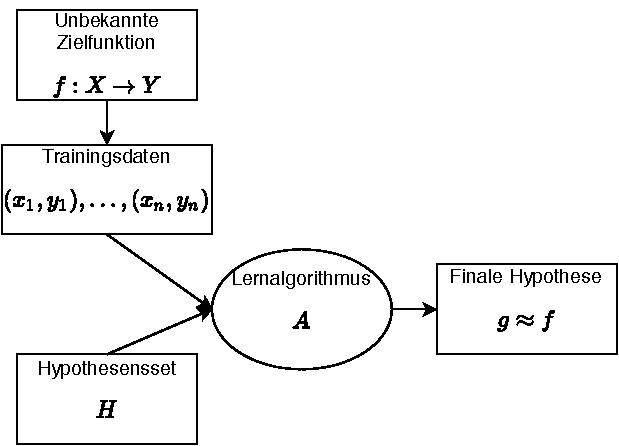
\includegraphics[scale=1]{pic/SupervisedLearning.pdf}
		\caption[Darstellung von überwachtem Lernen]{Darstellung von überwachtem Lernen}
		\label{fig:supervisedLearning}
	\end{figure}

	
	Ein häufig beobachtetes Problem bei maschinellem Lernen ist das sogenannte Overfitting, auf Deutsch Überanpassung, wenn das Modell zwar die Trainingsdaten gut approximiert, aber keine gute Generalisierung für unbekannte Daten bildet, d.\,h. zu stark an die Trainingsdaten angepasst ist. Gründe dafür können eine zu hohe Komplexität des Lernmodells wie z.\,B. zu viel Training oder zu wenig Trainingsdaten sein. %TODO: Satz fixen
	In beiden Fällen wird ungewollt ein Teil des \textit{noise} %TODO: evtl. einführen
	der Trainingsdaten in das Modell übernommen. Das Gegenteil von Overfitting ist Underfitting, das den Fall beschreibt, in dem das Modell die Beziehung von Merkmalen und Ziel nicht ausreichend erfasst. Dies ist unter anderem der Fall, wenn die zum Training verwendete Stichprobe verzerrt ist.
	
	Zum Prozess des maschinellen Lernens gehört ebenfalls das Sammeln der Daten und die Transformation in Merkmale, die dem Lernalgorithmus als Eingabe dienen. Dieser Prozess ist entscheidend für den Erfolg des Lernprozesses, da nur aus aussagekräftigen Daten ein gutes Modell erzeugt werden kann.

	\subsection{Evaluation und Validierung}
	
	Ein erzeugtes Modell muss in jedem Fall auf Daten validiert werden, mit denen nicht trainiert wurde, um den Fehler auf unbekannten Daten abschätzen zu können. Eine Möglichkeit, dies zu tun, bietet die Hold-Out-Validierung, bei der die Daten zufällig in Trainings- und Testset aufgeteilt werden. Das Modell wird mit dem Trainingsset aufgebaut und auf dem Testset getestet und evaluiert. Eine andere übliche Technik ist die Kreuzvalidierung, bei der die Daten auf $v $ gleich große Mengen, im Englischen \textit{folds}, verteilt werden. Anschließend werden $v$ Modelle trainiert, wobei jeweils eine Menge ausgelassen wird, auf der anschließend getestet wird. %TODO: Satz verständlicher
	Bei einer extremen Variante, der Leave-One-Out Kreuzvalididierung entspricht $v$ der Anzahl der Datenpunkte. Üblich ist jedoch $v$-fache Kreuzvalidierung mit $v=5$ oder $v=10$, auch abhängig von der Datenmenge und der verfügbaren Rechenleistung.
	
	Neben der Validierung des finalen Modells müssen auch bei der Modellauswahl Entscheidungen getroffen werden, vor allem, welches Modell und welche Hyperparameter gewählt werden. Hyperparameter sind Parameter von Modellen maschinellen Lernens, die vor dem Training des Modells festgelegt werden und die Modellarchitektur bestimmen oder den Lernalgorithmus betreffen. Da auch die Wahl dieser validiert werden muss, werden insgesamt drei Datensets benötigt: Trainings-, Validierungs- und Testset, da sonst die Wahl der Hyperparameter durch das Testset beeinflusst würde und kein unabhängiger Test mehr möglich wäre. Das Testset wird also erst genutzt, nachdem alle Entscheidungen getroffen wurden. Typisch ist ein Hyperparameter-Tuning durch Kreuzvalidierung auf dem Trainingsset mit einem anschließenden Retraining mit den ermittelten Parametern auf dem gesamten Trainingsset. Der Ablauf ist in Abbildung \ref{fig:validation-ablauf} visualisiert.
	
	\begin{figure}[H]
		\centering
		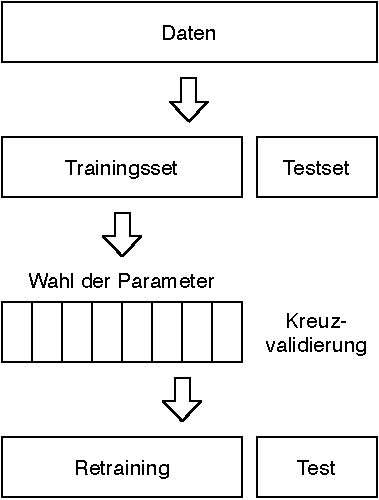
\includegraphics[scale=1]{pic/validation-ablauf.pdf}
		\caption{Ablauf von Training und Validierung}
		\label{fig:validation-ablauf}
	\end{figure}
	
	Um die Auswahl für ein Modell treffen zu können, werden Evaluationsmetriken benötigt. Für diese werden im Folgenden die englischen Bezeichnungen verwendet, da diese auch im Deutschen geläufiger sind.
	
	Vor allem für die Bewertung binärer Klassifikationen gibt es verschiedenste Metriken, die die richtigen und falschen Klassifikationen miteinander gewichten. Dafür wird bei positiv klassifizierten Datenpunkten zwischen Richtig-Positiven TP und Falsch-Positiven FP unterschieden; bei den negativ klassifizierten zwischen Richtig-Negativen TN und Falsch-Negativen FN. Eine Darstellung dieser vier nennt man Confusion Matrix. Diese ermöglicht eine erste Einschätzung der Fehlerverteilung. Ein häufig verwendetes und einfaches Gütemaß ist die Accuracy $\text{ACC} = \frac{TP + TN}{TP + TN + FN + FP}$, die allerdings bei ungleich großen Klassen problematisch ist, da eine hohe Genauigkeit erreicht wird, wenn immer die größere Klasse vorausgesagt wird. In diesem Fall kann auch die Balanced Accuracy verwendet werden, die dieses Ungleichgewicht einbezieht:
	\[
		\text{balanced-accuracy} = \frac{1}{2}\left( \frac{TP}{TP + FN} + \frac{TN}{TN + FP}\right).
	\]
	 Bei der Precision, auch Positive Predictive Value, $\text{PPV} = \frac{TP}{TP + FP}$ werden falsch-positive Klassifikationen \glqq bestraft\grqq{}; beim Recall, der \acl{TPR} $\text{TPR} = \frac{TP}{TP + FN}$, auch Sensitivity genannt, falsch-negative Klassifikationen. Letztere werden oft in einem Maß zusammengefasst, dem F1-Score, der das harmonische Mittel aus beiden bildet:
	\[
		F_1 = 2 \cdot \frac{\text{PPV} \cdot \text{TPR}}{\text{PPV} + \text{TPR}}.
	\]
	
	Eine weitere Möglichkeit, die Qualität eines binären Klassifikators zu evaluieren, ist die \ac{ROC} Kurve, bei der die \ac{TPR}, also der Recall, und die \ac{FPR} gegeneinander aufgetragen werden und so den Kompromiss zwischen \ac{TPR} und \ac{FPR} abhängig vom Schwellwert zeigt. Die Fläche unter dieser Kurve, die \ac{AUC}, beschreibt, wie gut das Modell die beiden Klassen trennt. Eine perfekte Trennung führt zu $\text{AUC} = 1$.
	
	Bei einer Regression werden üblicherweise der \ac{MAE} oder der \ac{MSE} betrachtet, die die Größe des Fehlers von dem vorhergesagten $\hat{y}$ im Vergleich zur Zielgröße $y$ ausdrücken und wie folgt berechnet werden:
	\begin{align*}
		\text{MAE}(y, \hat{y}) &= \frac{1}{n_{\text{samples}}} \sum_{i=0}^{n_{\text{samples}}-1} \left| y_i - \hat{y}_i \right| \\
		\text{MSE}(y, \hat{y}) &= \frac{1}{n_\text{samples}} \sum_{i=0}^{n_\text{samples} - 1} (y_i - \hat{y}_i)^2		
	\end{align*}
	
	Die Auswahl der betrachteten Metriken ist von dem vorliegenden Problem abhängig. %TODO: mehr Inhalt in Sätzen ist cool

	\subsection{Lernmodelle und deren mathematischer Hintergrund}
	
		Es gibt eine Vielzahl von Modellen des maschinellen Lernens, von denen eine Auswahl in dieser Arbeit betrachtet und vorgestellt wird. Alle verallgemeinern eine Verteilung von Trainingsdaten und haben das Ziel, eine Funktion $g$ zu finden, die $f$ approximiert und mit der die Zielgröße $y$ vorhergesagt werden kann. Bei einer Klassifikation sollen die verschiedenen Klassen möglichst genau separiert und bei einer Regression der Wert möglichst genau vorhergesagt werden. Diese Funktion wird auch Entscheidungsfunktion genannt und minimiert eine gewählte Kostenfunktion, die beschreibt, wie sehr die Vorhersagen von der Zielgröße abweichen. Bei linearen Modellen beispielsweise ist die Vorhersage mit $\hat{y}_i = \theta x_i$ eine lineare Kombination der gewichteten Merkmale für Datenpunkt $x_i \in X$. $\hat{y}_i$ kann dabei entweder direkt die Vorhersage eines Wertes sein oder genutzt werden, um eine Klassenzugehörigkeit zu ermitteln. Bei einer binären Klassifikation kann dafür beispielsweise die Signum- oder die logistische Funktion mit einem Schwellwert genutzt werden. Die genutzte Funktion wird auch Aktivierungsfunktion genannt. Die Parameter der Entscheidungsfunktion, in diesem Fall die Koeffizienten des Merkmalsvektors, werden im Nachfolgenden allgemein $\theta$ genannt. Sie sind der Teil der Entscheidungsfunktion, der von den Daten gelernt werden muss.
		
		Während des Trainings werden die besten Parameter $\theta$ ermittelt. Dafür wird eine Funktion benötigt, die ausdrückt, wie gut das Modell den Trainingsdaten angepasst ist. Diese besteht allgemein aus zwei Teilen: der Kostenfunktion $L$ und der Regularisierung $\Omega$:
		
		\[
			C(\theta)= L(\theta) + \Omega(\theta)
		\]
		
		Als Kostenfunktion wird vor allem für Regressionsprobleme häufig der \ac{MSE} verwendet. Bei binären Klassifikationsproblemen kann aber beispielsweise auch die Anzahl der falschen Klassifikationen verwendet werden. Die Regularisierung kontrolliert die Komplexität des Modells, um Overfitting zu vermeiden. Das Ziel des Trainings ist es demnach, die Anpassung des Modells zu optimieren, also $C$ zu minimieren. Dieses Minimierungsproblem wird abhängig von dem verwendeten Modell gelöst. Bei einer linearen Regression beispielsweise kann die Methode der kleinsten Quadrate verwendet werden, um die Fehlerquadrate zu minimieren, da eine Regularisierung bei einem linearen Modell nicht nötig ist. Der Gewichtungsvektor $\theta$ kann hier durch direktes Auflösen berechnet werden:
		\[
			\argmin_{\theta} \sum_{i=1}^{n} (\theta^T x_i - y_i)^2
			\Rightarrow \theta = (X^T X)^{-1} X^Ty
		\]
		
		Bei komplexeren Minimierungsproblemen ist die Methode kleinster Quadrate nicht ausreichend und es werden andere Methoden zur Fehlerminimierung benötigt. Eines davon ist das Gradientenabstiegsverfahren, bei dem in jedem Schritt die Ableitung der Kostenfunktion nach jedem der Gewichte berechnet wird und der Schritt gewählt wird, der die Funktion am stärksten minimiert.
		
		Eine andere Möglichkeit ist, nicht linear separierbare Daten mit dem sogenannten Kerneltrick linear separierbar zu machen, statt nicht-lineare, komplexere Verfahren zu verwenden. Dabei wird durch Ersetzen des Skalarproduktes implizit der Variablenraum transformiert. Ein Beispiel ist der Gaußsche RBF-Kernel, wobei RBF für radial basis function steht. Sind $x$ und $x'$ Merkmalsvektoren, ist der RBF-Kernel wie folgt definiert:
		\[
			K_{RBF} (x, x\prime) := \text{exp}(-\gamma \|x - x\prime\|^2) \text{ mit } \gamma > 0
		\]
		In der Transformation werden alle Nicht-Linearitäten berücksichtigt, wodurch anschließend Linearität möglich ist. %TODO: besser formulieren
		
		Im Folgenden werden die in dieser Arbeit genutzten Modelle näher vorgestellt. Die Nachimplementierung von existierenden Algorithmen umfasst außerdem drei Modelle, die hier nicht detailliert vorgestellt werden: die \ac{SVM}, die \ac{LDA} und das \ac{MLP}. Wichtig für die Einordnung ist, dass es sich bei \ac{LDA} und \ac{SVM} um zunächst lineare Modelle handelt und die \ac{SVM} häufig mit dem Kerneltrick verwendet wird, um die Daten zu transformieren. Beim \ac{MLP} handelt es sich um ein Neuronales Netz, das Nichtlinearität ermöglicht.

	
		\subsubsection{Classification And Regression Trees}
		
		\ac{CART} sind nicht-lineare Modelle, die einem Binärbaum entsprechen. Sie können sowohl für Regression als auch für Klassifikation verwendet werden. Zwar sind sie hinsichtlich ihrer Performance oft anderen Lernmodellen unterlegen, werden aber als Teil von komplexeren Modellen genutzt und haben den Vorteil, sehr gut nachvollziehbar zu sein. Im Gegensatz zu vielen anderen Modellen benötigen sie keine Normalisierung der Merkmale. Es wird ein Pfad in einem Baum durchlaufen, indem an jedem Knoten unterschieden wird, ob ein bestimmtes Merkmal über oder unter einem Schwellwert liegt. Die Kostenfunktion bei einer Regression ist in der Regel der \ac{MSE}. Für die Kostenfunktion einer Klassifikation wird häufig die \glqq{}Reinheit\grqq{} eines Knoten $m$ gemessen. Sie beschreibt, wie deutlich die Mehrheit einer einzelnen Klasse in $m$ ist.
		
		Für den Aufbau eines \ac{CART} wird häufig das zu den greedy Algorithmen gehörende rekursive binäre Teilen verwendet. Hierbei wird ein Baum von der Wurzel zu den Blättern hin aufgebaut. In jedem Schritt wird das Merkmal gewählt, mit dem sich die Daten zu diesem Zeitpunkt am besten separieren lassen und der Schwellwert ermittelt. Abbruchkriterien sind unter anderem eine maximal erlaubte Tiefe oder eine Mindestanzahl von Datenpunkten in einem Blatt. Wenn diese zu viel Spielraum erlauben, neigen Bäume zum Overfitting.
		
		\subsubsection{Random Forest}
		
		Ein Zusammenschluss aus mehreren unkorrelierten Bäumen wird \acf{RF} genannt. Jeder dieser Bäume ist ein eigenständiges Modell, das ein Ergebnis liefert. Aus der Menge der Einzelergebnisse wird das endgültige Ergebnis ermittelt. Dadurch wird ein Teil der Nachvollziehbarkeit von Bäumen gegen eine bessere Generalisierung eingetauscht. Die einzelnen Bäume werden zufällig erzeugt, indem für jeden Baum $n$ zufällige Datenpunkte ausgewählt werden. Von $M$ Merkmalen werden nun $m \ll M$ ebenfalls zufällig gewählt, die als Kriterium für den Aufbau des Baumes verwendet werden. Der darauf folgende Aufbau des Baumes entspricht dem zuvor beschriebenen. Bei einer Klassifikation ist das endgültige Ergebnis je nach Implementierung ein Mehrheitsentscheid oder eine Kombination aller Wahrscheinlichkeiten; bei einer Regression der Durchschnitt aller Werte.
		
		Ein Random Forest hat gegenüber anderen Modellen den Vorteil, dass er sehr schnell trainiert und somit sehr effizient für große Datenmengen ist. Gleichzeitig kann das Ergebnis relativ einfach nachvollzogen werden.
		
		\subsubsection{Gradient Boosted Trees}
		
		Auch ein Gradient Boosted Tree kombiniert mehrere einfache Bäume. Im Gegensatz zum \ac{RF} hängt beim Gradient Boosted Tree jeder Baum von früheren Bäumen ab. Gestartet wird mit einem Baum, auf dessen Ergebnissen aufgebaut wird. Das endgültige Ergebnis wird auch hier aus der Menge an einzelnen Ergebnissen ermittelt, aber folgende Bäume konzentrieren sich jeweils darauf, die Schwächen der schon erzeugten Modelle auszugleichen.
		
		Auch Gradient Boosted Trees ermöglichen eine nachvollziehbare Entscheidung. Meist erreichen sie etwas bessere Ergebnisse als die einfacheren \acl{RF}s.

\section{Medizinische Grundlagen}\label{med-grundlagen}

Die vorliegende Arbeit beschäftigt sich mit der Beurteilung der Signalqualität in ballistokardiographischen Signalen. Zum Verständnis der gemessenen Vorgänge und der Problematik in Bezug auf die Signalqualität und dessen Beurteilung ist grundlegendes medizinisches Wissen über die gemessenen Vorgänge und messtechnisches Verständnis nötig. Aufgrund dessen wird hier eine kurze Übersicht über die medizinischen Grundlagen gegeben.

	\subsection{Kardiorespiratorisches System}
	
	Das kardiorespiratorische System (zusammengesetzt aus \textit{kardìa}, deutsch \glq Herz\grq{} und \textit{respiratio}, deutsch \glq Atmung\grq) setzt sich aus zwei Teilsystemen zusammen, dem kardiovaskulären und dem respiratorischen System, die zusammen die Versorgung der Organe mit Sauerstoff sicherstellen.
	
	Das kardiovaskuläre System umfasst das Herz, die Arterien und die Venen. In einem Zyklus wird das sauerstoffreiche Blut von der linken Herzkammer durch die Arterien zu den Organen gepumpt, wo sich der Sauerstoff zur Versorgung dieser vom Blut löst. Die Venen transportieren das nun kohlstoffdioxidreiche Blut in die rechte Herzkammer. Von dort wird es zur Lunge geführt, mit Sauerstoff angereichert und in die linke Herzkammer geleitet. Von dort beginnt der Vorgang von Neuem. Die Herzfrequenz ist hierbei ein relevanter messbarer Vitalparameter.
	
	Ein Herzschlag selbst besteht aus zwei Phasen: einer füllenden und einer auswerfenden Phase. Während der Diastole, der Erschlaffungs- und Bluteinströmungsphase, füllen sich die Herzkammern mit Blut. Diese Phase endet mit dem Schließen der Herzklappen und die Systole beginnt. Die Systole ist die Anspannungs- und Blutausströmungsphase: Die Herzklappen öffnen sich durch Kontraktion des Herzmuskels und das Blut kann ausströmen.
	
	Das respiratorische System umfasst die Lungen und den Lungenkreislauf. In einem Atemzyklus wird durch gezielte Muskelbewegungen Luft aus der Umgebung eingeatmet. Mit dem eingeatmeten Sauerstoff wird sauerstoffarmes Blut angereichert und anschließend die nun sauerstoffarme Luft ausgeatmet. In diesem Zusammenhang ist der Vitalparameter der Atemfrequenz messbar.

	\subsection{Übersicht Messtechniken}
	
	Zur Untersuchung der in dieser Arbeit betrachteten \acf{BKG} wird diese oft mit anderen Messmethoden als Referenz aufgenommen. Im Folgenden werden diese zur Einordnung kurz vorgestellt. \ac{BKG} selbst wird im nächsten Abschnitt separat betrachtet.
	
	Die \acf{EKG} zeichnet die elektrischen Aktivitäten des Herzmuskels auf, indem mit mehreren Elektroden die Spannungsänderung gemessen wird. Hier ist die Herzfrequenz sehr gut ablesbar.
	
	Die \acf{PPG} ist ein optisches Messverfahren, bei dem die Menge des von der Haut reflektierten bzw. transmittierten Lichtes gemessen wird. Dadurch kann die Änderung des Blutvolumens gemessen werden; die Lichtmenge nimmt bei Durchlaufen einer Pulswelle durch die Arterie deutlich ab. Dieses Signal bietet Rückschluss auf Atmung und Herzschlag. % TODO: evtl. rausnehmen
	
	Oft gemeinsam mit dem \ac{BKG} betrachtet wird die \acf{SKG}, bei der die Vibration der Wand des Brustkorbs, die durch den Herzschlag entsteht, aufgezeichnet wird. Aufgrund von fehlenden einheitlichen Definitionen wird in der Literatur teils auch der Begriff \ac{BKG} für \ac{SKG} genutzt.\footcite[Vgl.][]{Inan2015}

	\section{Ballistokardiographie}\label{ballistokardiographie}
	
	Im Folgenden wird die \acl{BKG} eingeführt. Diese Einführung beinhaltet den medizinischen und technischen Hintergrund, das Einsatzgebiet und die Signaleigenschaften.
	
	\subsection{Medizinischer und technischer Hintergrund}
	
	Ballistokardiographie (zusammengesetzt aus altgriechisch \textit{ballein}, deutsch \glq werfen\grq, \textit{kardía}, deutsch \glq Herz\grq{} und \textit{graphein}, deutsch \glq schreiben\grq) ist die graphische Darstellung der wiederholten, durch den Herzschlag verursachten Bewegungen des menschlichen Körpers. Erstmals schon im 19. Jahrhundert beobachtet\footcite[Vgl.][]{Gordon1877}, ermöglicht der technische Fortschritt in der Sensortechnik heute aussagekräftige Messungen. Das \ac{BKG} liefert durch die Aufzeichnung von zirkulierendem Blut und mechanischer Herzaktivität Informationen über die Gesamtleistung des kardiovaskulären Systems.\footcite[Vgl.][]{Pinheiro2010} Konkret gemessen wird eine Massenbewegung, die durch die schnelle Beschleunigung des Blutes entsteht, wenn es während des Herzschlages durch die großen Arterien bewegt wird: Bei der Verteilung des Blutes in die peripheren Blutgefäße verschiebt sich das Zentrum der Körpermasse in Richtung der Füße und während der atrialen Systole Richtung Körpermitte. Die \ac{BKG}-Wellenform entsteht durch diese Schwerpunktverschiebung.
	
	Die Messung dieser Bewegung ist mit verschiedenen Sensortypen, die z.\,B. hydraulisch oder elektromechanisch auf Druck reagieren, möglich. Sensoren können unter anderem in Waagen, Stühlen und Betten eingebaut werden. Besonders bei im Bett gemessenen Signalen kann oft nicht klar zwischen \ac{SKG} und \ac{BKG} unterschieden werden, da sich myokardiale Vibrationen und Massverschiebungen durch den Blutfluss überlagern. Diese gemischten Signale werden in der Literatur teils auch als \textit{cardiac vibration signals} bezeichnet.\footcite[Vgl.][]{Bruser2013} Da im Bereich der Signalverarbeitung oft nicht zwischen reinem \ac{BKG} und gemischten Signalen unterschieden wird, wird dies in der vorliegenden Arbeit ebenfalls nicht. %TODO: wird nach dem Komma ersetzen
	
	Verschiedene Studien kommen zu unterschiedlichen Ergebnissen bezüglich der Frage, welchen kardiovaskulären Ursprung die einzelnen Signalteile haben. Aufgrund dessen gestaltet sich die detaillierte Interpretation des \ac{BKG}-Signals als schwierig. Da es neben Informationen zur \ac{HR} und \ac{HRV} ein genauerer Indikator für das Alter des Herzens als Lebensalter ist, hat es trotzdem klinische Relevanz. Außerdem lassen sich durch abnormale Ballistokardiogramme Herzerkrankungen voraussagen, bevor Symptome auftreten. Besonders bei älteren Personen sind diese also eine wichtige Warnung.\footcite[Vgl. zu diesem Absatz][]{Pinheiro2010}
	
	\subsection{Einsatzgebiet}
	
	Durch diese Beschreibung wird deutlich, dass \ac{BKG} anders als die sehr bekannte \ac{EKG} ist. Der entscheidende Vorteil der \ac{BKG}s liegt darin, dass kein einschränkender Körperkontakt durch z.\,B. aufgeklebte Elektroden nötig ist: Es lässt sich in Alltagsgegenständen wie Stühlen aber vor allem auch Betten implementieren, ohne dass es während der Messung zu Einschränkungen im alltäglichen Leben kommt oder medizinisches Fachpersonal anwesend sein muss. Damit gehört es zu den \textit{unobtrusive} Messmethoden und eignet sich gut zur Langzeit- und Trendbeobachtung des Gesundheitszustandes - sowohl im klinischen Kontext als auch Zuhause. Besonders für Patient*innen mit chronischen Krankheiten und zur Früherkennung krankhafter Veränderungen bietet eine gesundheitliche Überwachung von Zuhause großes Potential.\footcite[Vgl.][]{Inan2015} Je nach Aufbau des Messsystems verändert sich auch die Art der Informationen, die aus dem \ac{BKG}-Signal gewonnen werden können. Sehr genaue, kontrolliert aufgenommene \ac{BKG}-Signale ermöglichen eine aussagekräftige Analyse der Morphologie wobei beispielsweise in Betten eingebautes \ac{BKG} zunächst nur Aussagen zu Herzrate und Herzratenvariabilität bietet. Zusätzlich zu Informationen der Herzaktivitäten ermöglichen Bettsysteme aber auch Informationen über das allgemeine Aktivitätslevel und somit auch über die Schlafqualität. \footcite[Vgl.][]{Bruser2011} In dieser Arbeit wird es um die Aufzeichnung von \ac{BKG}-Signalen in Betten gehen. Der Aufbau eines solchen Bettsystems ist in Abbildung \ref{fig:bcgbed} gezeigt.
	
	 \begin{figure}[H]
	 	\centering
		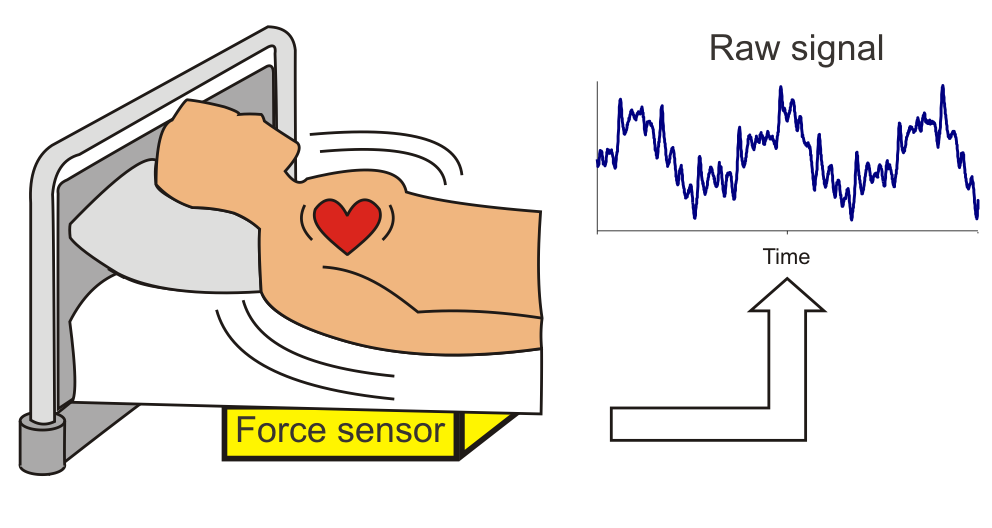
\includegraphics[width=0.7\textwidth]{pic/bcgBed.png}
		\caption[Übersicht über die Funktionsweise eines allgemeinen im Bett eingebetteten \ac{BKG}-Systems]{Übersicht über die Funktionsweise eines allgemeinen im Bett eingebetteten \ac{BKG}-Systems.\protect\footnotemark}
		\label{fig:bcgbed}
	\end{figure}
	\footnotetext{Entnommen aus \cite{Bruser2011}}
	
	Allerdings ergeben sich neben diesen umfassenden Möglichkeiten auch Nachteile gegenüber konventionellen Messmethoden. Die größte Herausforderung ist eine stark variierende Signalqualität, die sich durch das unkontrollierte Umfeld und die Art der Messung ergibt.

	\subsection{Signaleigenschaften}
	
	Das gemessene \ac{BKG}-Signal setzt sich aus Herzaktivitäten, Atmungsaktivitäten und Körperbewegungen zusammen. Gegebenenfalls wird es noch durch Störungen der Messung beeinflusst. Bei einer gesunden Person ohne Störeinflüsse wird die in Abbildung \ref{fig:bcgwaveform} abgebildete Wellenform erwartet. Diese Idealform lässt sich in 3 Gruppen unterteilen: Die präsystolische, wobei diese häufig nicht beachtet wird, die systolische und die diastolische Gruppe. Die mit H bis K markierten Extremwerte gehören bei dieser Unterteilung zur systolischen Gruppe, die Wellen L bis N zur diastolischen Gruppe. Die präsystolische Gruppe, die aus den Wellen F und G besteht, ist in hier nicht abgebildet. I und J werden auch als \textit{ejection waves} bezeichnet. In Bezug auf andere Messmethoden ist zu bemerken, dass die H-Welle nahezu synchron mit dem ersten Herzgeräusch ist. Der Abstand des R-Peaks, des Hochpunkts eines \ac{EKG}s, zur H-Welle variiert im Bereich von \numrange{0,2}{0,3} Sekunden.\footcite[Vgl.][]{DELALLA1950} Die Amplitude der Wellen ohne Störeinflüsse ist hauptsächlich abhängig von dem Herzzeitvolumen, der Herzkraft und der Geschwindigkeit des Auswurfs.\footcite[Vgl.][]{Pinheiro2010}
	
	\begin{figure}[H]
		\centering
		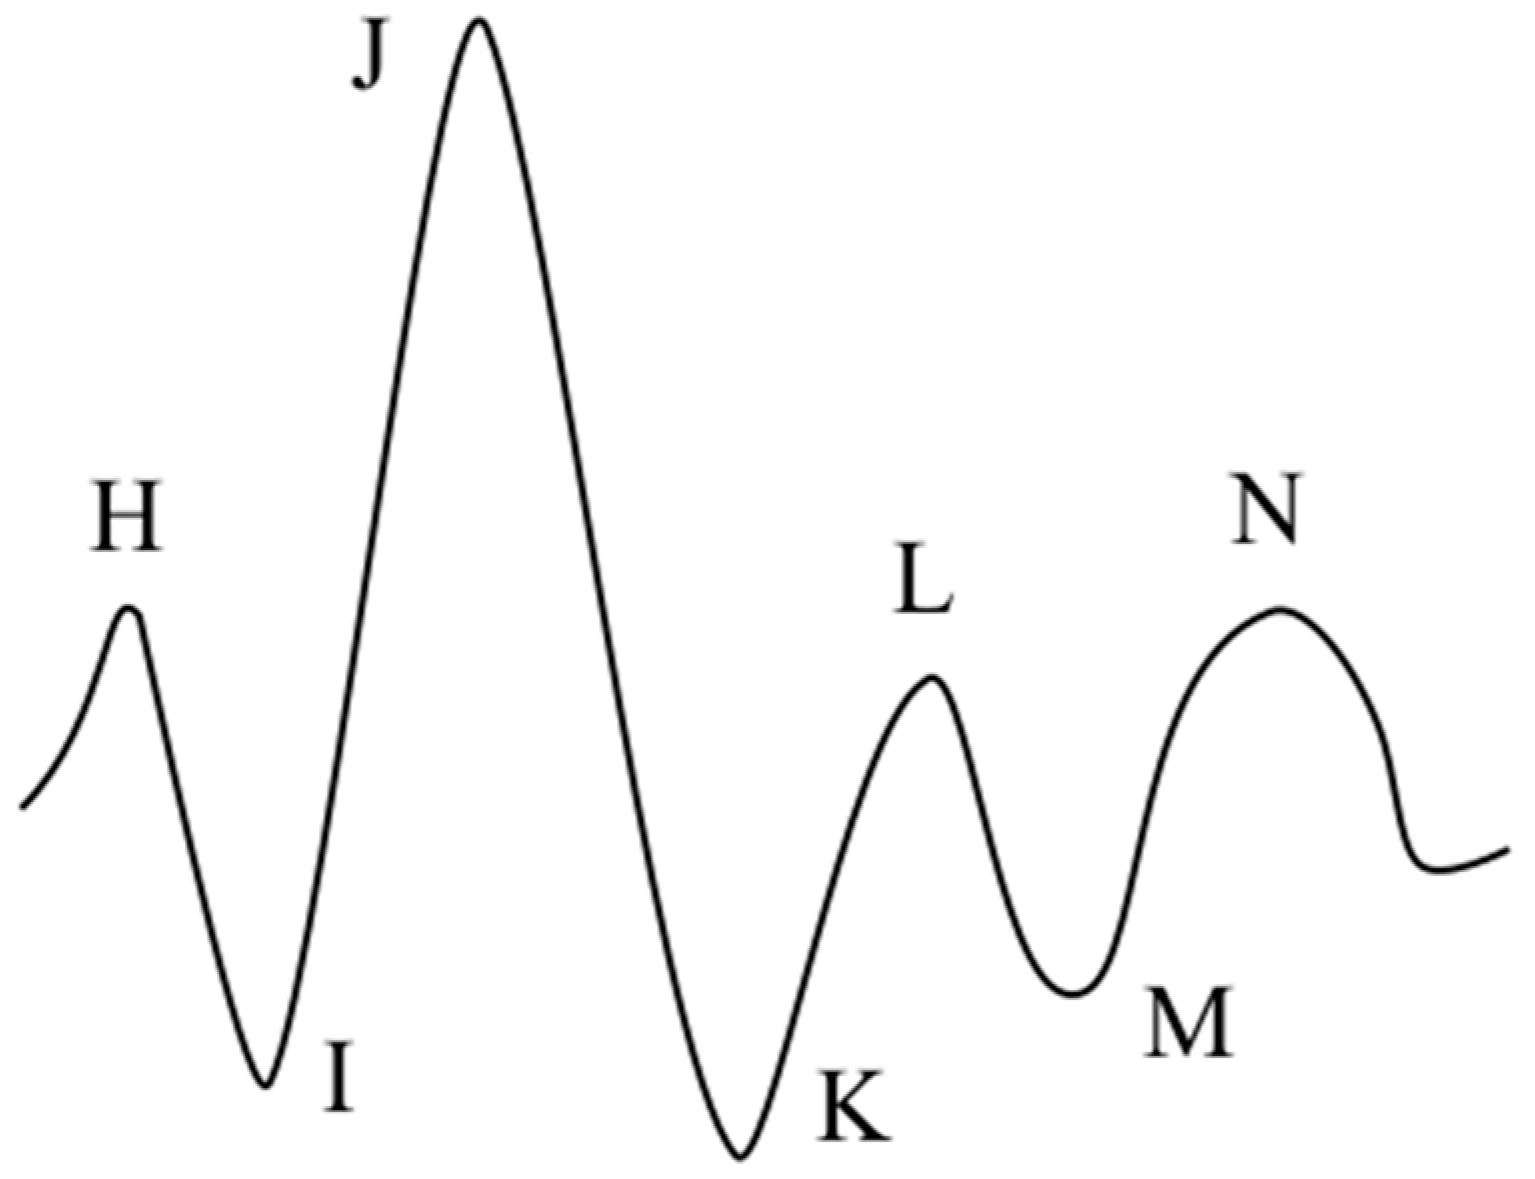
\includegraphics[width=0.7\textwidth]{pic/bcgWaveform.png}
		\caption[Beispiel eines typischen \ac{BKG}-Signals mit Nomenklatur]{Beispiel eines typischen \ac{BKG}-Signals mit Nomenklatur\protect\footnotemark}
		\label{fig:bcgwaveform}
	\end{figure}
	\footnotetext{Entnommen aus \cite{Albukhari2019} nach \cite{Starr1939}.}
	
	Im Idealfall wird zwar die oben beschriebene Wellenform erwartet, bei der die Wellen H bis L eine deutliche W-Form bilden, allerdings ist es trotz dieser typischen Form selten, dass alle nicht-systolischen Komponenten sichtbar sind.\footcite[Vgl.][]{Pinheiro2010} Es gibt eine starke Variation der Signalmorphologie sowohl zwischen als auch innerhalb von Individuen. Der größte Einfluss ergibt sich durch die verwendeten Sensoren und die Position der Person, also zum Beispiel ob im Stehen, Sitzen oder Liegen gemessen wird.\footcite[Vgl.][]{Sadek2019} Es gibt Studien, die zeigen, dass die intraindividuelle Varianz über serielle Messungen hinweg niedrig ist.\footcite[Vgl.][]{Inan2015} Allerdings gilt das nicht, wenn sich die Position der Person verändert. Hierbei reicht es schon, wenn die Person in Rückenlage statt Seitenlage liegt.\footcite[Vgl.][]{Bruser2011} Aufgrund dieser Variationen in der Signalmorphologie wurden schon in den 1950er Jahren drei Achsen für die Aufzeichnung des \ac{BKG}s definiert: Die longitudinale (Kopf-Fuß), die transversale (Seite-Seite) und die dorsoventrale (Rücken-Brust).\footcite[][Vgl.]{Bruser2011, Inan2015} Zu Beginn maßen die meisten Systeme entlang der longitudinalen Achse, die z.\,B. der Messung auf einer Waage entspricht. \textit{Unobtrusive} Messsysteme, wie die hier betrachtete Messung in Betten, messen entlang einer Kombination der transversalen und der dorsoventralen Achse - abhängig von der Position der Person. Besonders diese Kombination sorgt für eine große intra- und individuelle Variation des Signals. Abbildung \ref{fig:bcg2postures} verdeutlicht dies durch den direkten Vergleich von \ac{BKG}-Aufzeichnungen zweier Herzschläge von 2 Personen. Bei jeder dieser beiden Personen wurde in zwei verschiedenen Positionen gemessen.\footcite{Bruser2011} Auch der Ursprung des Signals ist abhängig von der Messachse. Bei longitudinal gemessenem \ac{BKG} ist der Einfluss des Herzzeitvolumens schon seit 1929 beobachtet.\footcite[Vgl.][]{Starr1939} Im Gegensatz dazu ist der Ursprung des in Betten gemessenen \ac{BKG}-Signals nicht genau bekannt. Das liegt unter anderem daran, dass mechanische Komponenten wie z.\,B. die Matratze einen schwer zu modellierenden Einfluss haben.
	
	\begin{figure}[H]
		\centering
		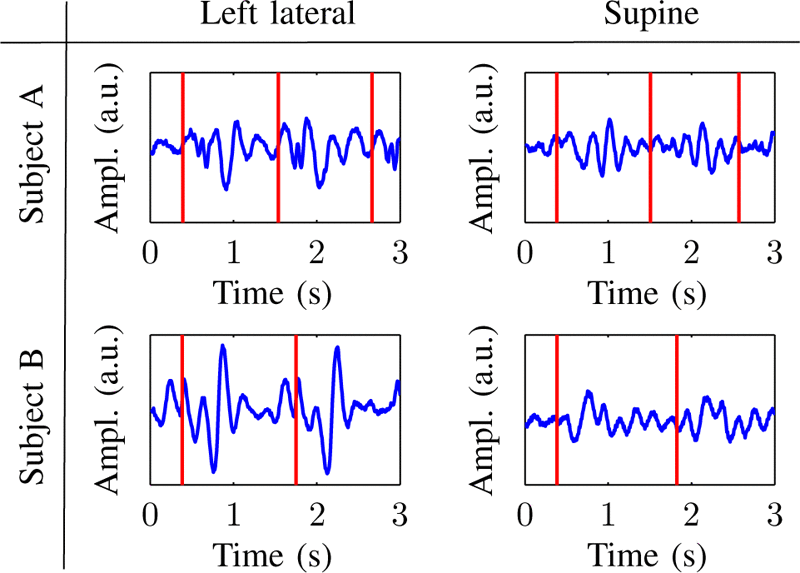
\includegraphics[width=0.7\textwidth]{pic/bcg2postures.png}
		\caption[\ac{BKG}-Aufnahmen in Rücken- und Seitenlage]{Hochpass-gefilterte \ac{BKG}-Aufnahmen von zwei Herzschlägen zwei verschiedener Personen, jeweils in Rücken- und Seitenlage gemessen. Die vertikalen Linien markieren die R-Peaks der EKG-Referenz.\protect\footnotemark}
		\label{fig:bcg2postures}
	\end{figure}
	\footnotetext{Entnommen aus \cite{Bruser2011}.}
	
	Neben Einflüssen der verwendeten Messachse und der Körperposition beeinflusst auch die Atmung die Signalform. Normale Atmung beeinflusst die Amplitude der \textit{ejection waves} I und J. Bei Atemstillstand dagegen werden die H und J Wellen verzerrt. Auch bei einer gesunden, sich nicht bewegenden Person, die ihre Atmung kontrolliert, wird kein exakt Schlag für Schlag reproduzierbares Signal erzeugt werden.\footcite[Vgl.][]{Pinheiro2010} Von \citeauthor{Zink2017} werden die Einflüsse der Atmung in der vertikalen Achse eines dorsoventralen \ac{BKG}s als große Schwingungen einer Wellenlänge von fünf bis zehn Sekunden beschrieben. Innerhalb dieser sind kleinere Schwingungen mit höherer Frequenz sichtbar, die jedoch keiner bestimmten Sequenz folgen.\footcite[Vgl.][]{Zink2017} Zusätzlich zu dieser schon beschriebenen Variabilität kommt es sehr leicht zum Entstehen von Artefakten. Ursprung ist entweder das Messsystem selbst oder Körperbewegungen. Insgesamt führt Bewegung der Patient*innen, auch die der Atmung, zu einem \textit{baseline drift}. Stärkere Bewegungen führen zu einer Massenverschiebung, die um ein Vielfaches größer als die gemessenen Vorgänge ist. Aufgrund dessen führt sie immer dazu, dass das Signal stark verzerrt oder sogar vollständig überlagert wird.

	
	Besonders im Vergleich zu anderen kardiorespiratorischen Signalen wie dem \ac{EKG} und \ac{PPG} wird deutlich, dass \ac{BKG}-Signale auch in konsekutiven Messungen deutlich variabler sind. Abbildung \ref{fig:variabilitaet} zeigt dies am Beispiel von \ac{BKG}-Aufnahmen eines im Bett integrierten Messsystems im Vergleich zum parallel aufgenommenen \ac{EKG}. Es zeigt sich, dass selbst nach Entfernung von Überlagerungen von Atmung  und Bewegung das \ac{BKG}-Signal eine höhere Variabilität in Bezug auf Amplitudenhöhe, Reihenfolge der Extremwerte und der gesamten Form aufweist.\footcite[Vgl.][]{Zink2017} Es wird allerdings angenommen, dass aufeinander folgende Herzschläge sich ähneln.\footcite[Vgl.][]{Bruser2013} Diese Eigenschaft wird Selbstähnlichkeit genannt. \citeauthor{Bruser2013} nennen als eine mögliche Ausnahme den Fall, dass ein unregelmäßiger Herzschlag mit sehr niedrigem Schlagvolumen einem regulären Herzschlag folgt. In dem Fall ist es möglich, dass die Amplitude im Vergleich so klein ist, dass sie verdeckt wird. Dies ist z.\,B. bei Vorhofflimmern möglich. Eine Untersuchung von \citeauthor{Rosales2012} zeigt dieses Verhalten der Selbstähnlichkeit nicht bei den kleineren Extremwerten die den Hochpunkt J umgeben. Dass die Ähnlichkeit um J am größten ist, zeigt auch Abbildung \ref{fig:variabilitaet}.
	
	\begin{figure}[H]
		\centering
		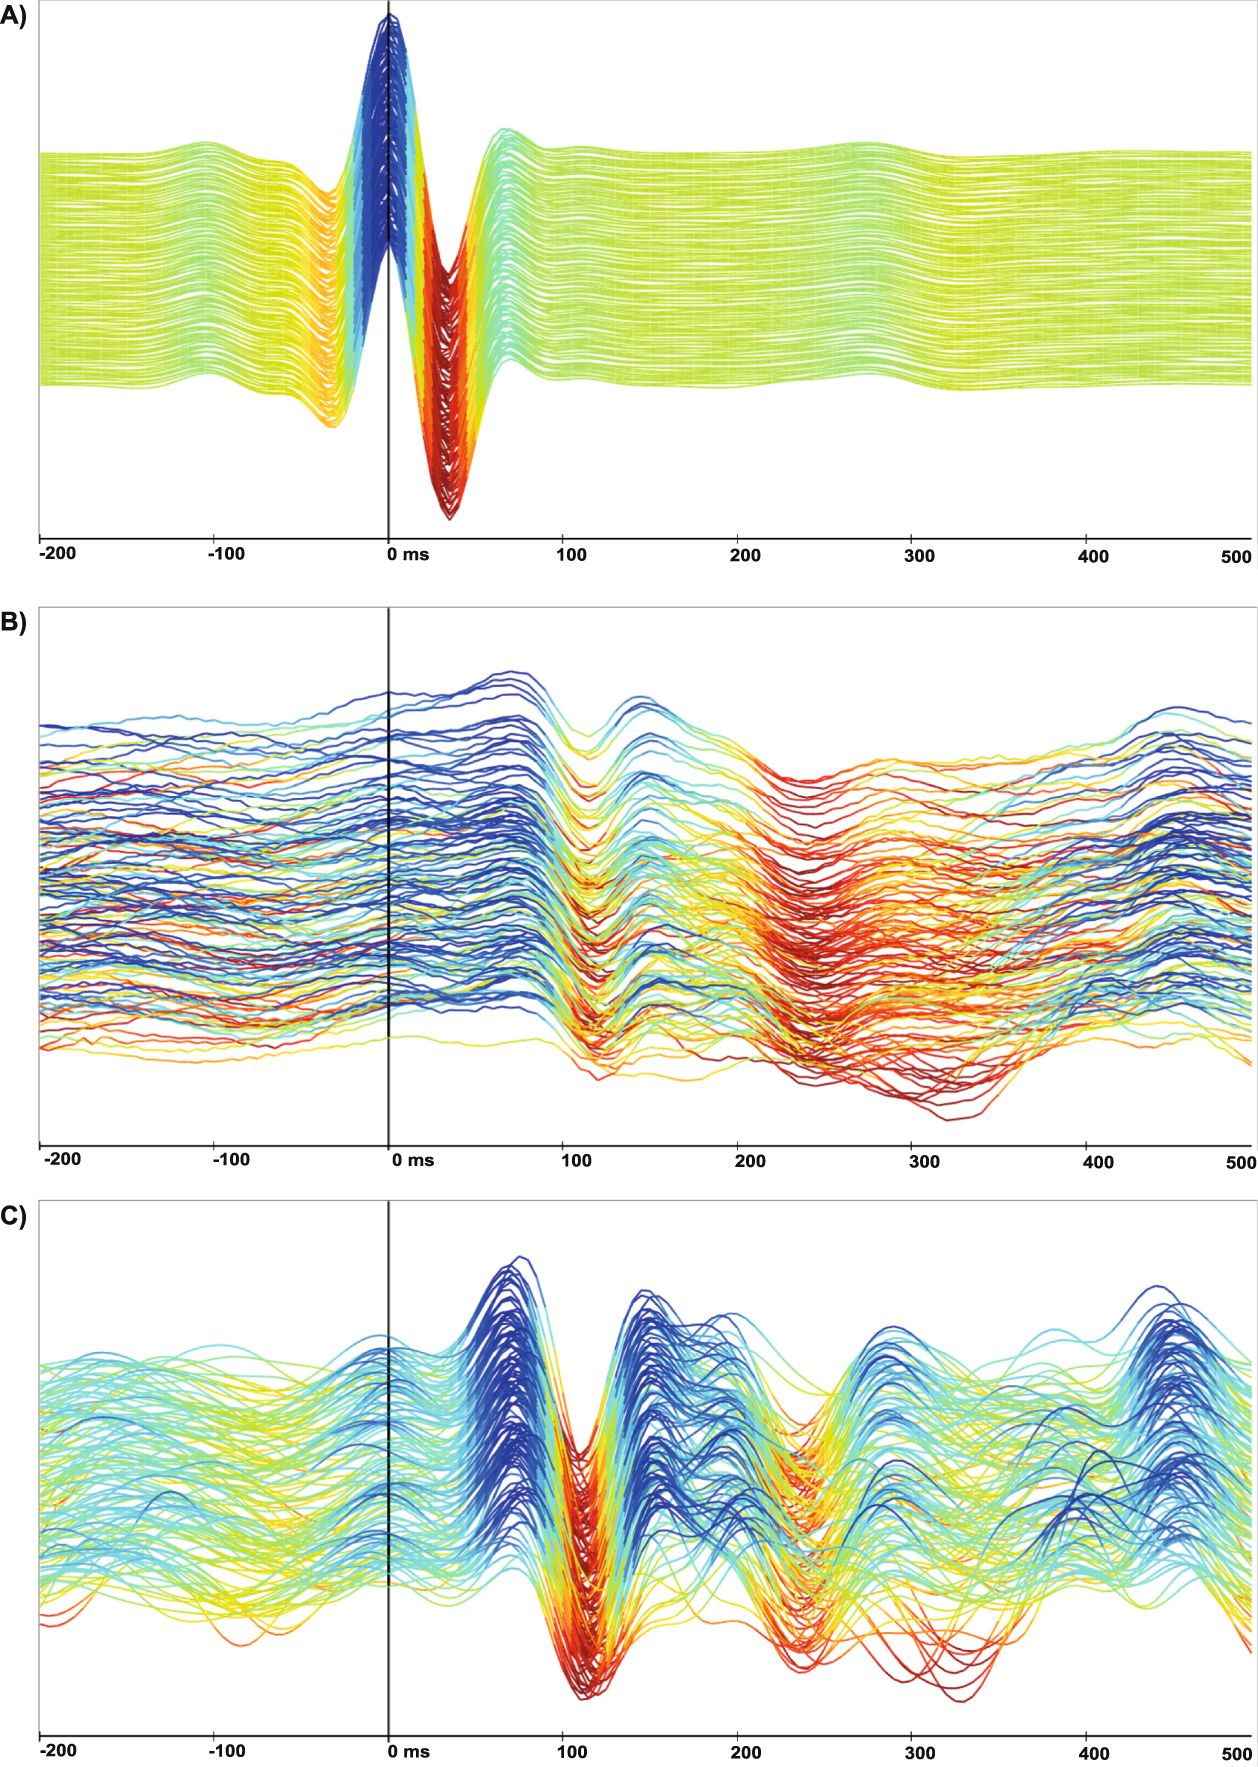
\includegraphics[width=0.6\textwidth]{pic/Variabilitaet.jpg}
		\caption[Visualisierung der Variabilität des \ac{BKG}-Signals]{Diagramm aus 128 konsekutiven Herzschlagen im EKG (A) und BKG (B,C), segmentiert durch das EKG. Die Farben dienen der besseren Visualisierung der Amplituden. (A) EKG-Signal; (B) BKG-Signal mit Überlagerungen durch Atmung und Bewegung; (C) \ac{BKG}-Signal ohne Bewegungsartefakte und Atmung.\protect\footnotemark}
		\label{fig:variabilitaet}
	\end{figure}
	\footnotetext{Entnommen aus \cite{Zink2017}.}
	
	
	Zusammengefasst lässt sich sagen, dass es sich bei ballistokardiographischen Signalen um nichtstationäre Signale handelt, deren Ursprung nicht genau bekannt ist. Die Signalform wird von der Messachse, der Position und Körperhaltung der Proband*innen und dem Messsystem selbst beeinflusst. Besonders bei dem hier im Fokus liegenden Anwendungsfall Bett kommt es sowohl durch die unkontrollierbare Umgebung als auch die Signaleigenschaften selbst zu einer starken Variation der Morphologie und vielen Artefakten im Signal. Trotz dieser Einschränkungen ist die \acl{BKG} eine Messtechnik, die sich einfach \textit{unobtrusive} in den Alltag einbauen lässt und Aussagen über die \acl{HR} und die \acl{HRV} ermöglicht.


\chapter{Signalverarbeitung bei ballistokardiographischen Signalen}

\section{Grundsätzliches}

\begin{itemize}
	\item Signale sind durch quasiperiodische Natur des Herzens selbst quasiperiodisch
	\item gleichzeitige Messung von zwei verschiedenen Vorgängen gleichzeitig
	\item Morphologie variiert im Verlauf eines Atemzyklus
	\item Filterung nach Frequenzen durch Bandpass-Filterung möglich
	\item Normbereich Atemfrequenz: 12 bis 25 Atemzüge pro Minute, ober- und unterhalb abnormal
	\item Herzfrequenz: 30 bis 210 Schläge pro Minute, dabei 30 Schläge pro Minute Pulsabsenkung nachts, Ruhepuls ist höher
	\item durch Eigenschaften von \ac{BKG}-Signalen schwieriger in Signalverarbeitung als andere kardiorespiratorische Signale
	\item \citeauthor{Paalasmaa2015} Zitat:
\end{itemize}

\begin{quote}\textit{The properties of the BCG signal vary so much in practice that no simple filtering rule can be devised for an accurate and reliable beat-to-beat interval detection}\footcite{Paalasmaa2015}\end{quote}

\begin{itemize}
	\item verschiedene Arten Signalverarbeitung: Arbeit im Zeitbereich, Arbeit im Frequenzbereich
	\item Zeitbereich: oft basierend auf existierendem Wissen über Morphologie des physiologischen Signals -> bei \ac{BKG} schwierig, da Morphologie sehr variabel
	\item frequenzbasiert: Analyse von spektralen Eigenschaften
	\item Analysen im Frequenzbereich erstmal nur durchschnittliche Frequenzen
	\item für einige medizinsche Anwendungen ausreichend, für andere, zB \ac{HRV} nicht
\end{itemize}

\section{Detektion von Herzschlägen}\label{CLIE}

	\begin{itemize}
		\item in dieser Arbeit Fokus auf von Brüser entwickelter Algoritmus, dem \textit{Continuous Local Interval Estimator}, kurz \textit{CLIE}
		\item in \ref{ballistokardiographie} erwähnte Annahme: aufeinander folgende Herzschläge ähneln sich
		\item Vorverarbeitung: Bandpass-Filter 0.5 und 20 Hz
		\item erste Ableitung des mit Savitzky-Golay gefilterten Signals für Analyse genutzte
		\item Algorithmus iteriert mit \textit{Moving Window} über das Signal
		\item 2 Schwellwerte genutzt, $T_min$ und $T_max$, basierend auf bekanntem Bereich der Herzrate
		\item Fensterlänge 2 mal maximale Intervalllänge \[w_i[v] = x[n_i + v], v \in \{ -T_{max} * f_s, ..., T_{max} * f_s\} \]
		\item adaptives Fenster schätzt nur Intervalllänge an Mittelpunkt des Fensters
		\item lokale Intervalllänge $T_i$ schätzen
		\item Zentrum des Analysefensters weiter bewegen $n_{i+1} = n_i + \Delta t * f_s$
		\item Schätzung der Intervalllänge durch drei Schätzer
	\end{itemize}
	
	\begin{align*}
		E\textsubscript{Corr}[n] &= \frac{1}{n} \sum_{v=0}^{n} w[v]w[v-n],\\
		E\textsubscript{AMDF}[n] &= (\frac{1}{n} \sum_{v=0}^{n} |w[v]-w[v-n]|)^{-1},\\
		E\textsubscript{MAP}[n] &= \max_{v \in \{0,...,n\}}(w[v]+w[v-n]).
	\end{align*}
	
	\begin{itemize}
		\item $E_{corr}$ berechnet eine modifizierte Autokorrelationsfunktion, mit $E_{AMDF}$ wird die Differenz des Signals zueinander miteinbezogen, AMDF steht für Modified average magnitude difference function
		\item mit $E_{MAP}$ werden die maximale Amplituden von beliebigen 2 Samples über das ganze Fenster berechnet, MAP steht für maximum amplitude pairs
		\item jeweils Wahrscheinlichkeitsfunktion, wie wahrscheinlich es ist, dass n dem tatsächlichen Schlag-zu-Schlag-Intervall entspricht
		\item Fusion dieser nach Bayes
	\end{itemize}
	\begin{align*}
		E_f[n] &= E\textsubscript{Corr}[n] \cdot E\textsubscript{AMDF}[n] \cdot E\textsubscript{MAP}[n],\\
		n_{opt} &= \argmax_{n} E_f[n]	
	\end{align*}
	
	\begin{figure}[H]
		\centering
		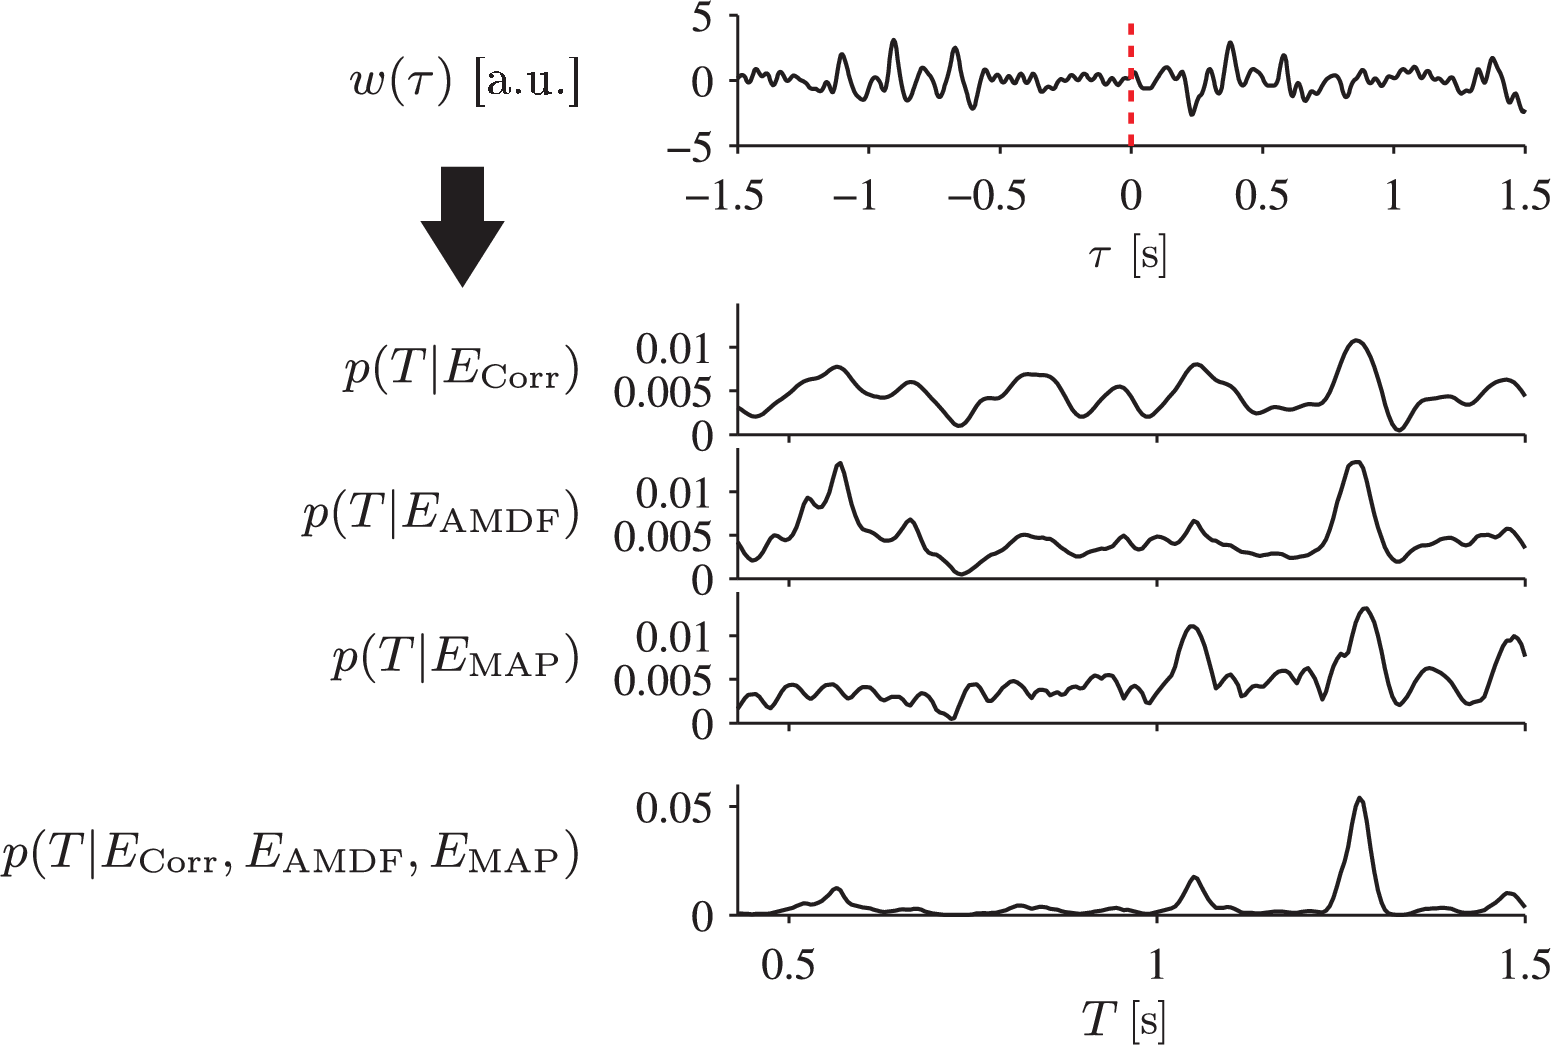
\includegraphics[width=0.7\textwidth]{pic/estimator-fusion.png}
		\caption[Intervallschätzer nach \citeauthor{Bruser2013}]{Die drei Intervallschätzer und ihre Fusionierung}
		\label{fig:estimator-fusion}
	\end{figure}
	
	\footcites[Vgl. zu diesem Absatz][]{Bruser2013}{Zink2017}

\section{Artefakterkennung}

	\begin{itemize}
		\item Artefakte = irrelevante Signalteile mit variierender Amplitude, Frequenz und Dauer, die physiologiches Signal stören \footcite{Nizami2013}
		\item Ziel Beurteilung Signalqualität: nur die Teile des Signals, die Vitalparameter enthalten verarbeiten
		\item Bewegungsartefakte, Sensorstörungen etc nicht verarbeiten
		\item Beispiele für Artefakte, einmal mit hoher, einmal mit niedriger Energie
	\end{itemize}
	
	\begin{figure}[H]
		\centering
		\includegraphics[width=0.7\textwidth]{pic/high-energy-artefacts.png}
		\caption[Intervallschätzer nach \citeauthor{Bruser2013}]{Die drei Intervallschätzer und ihre Fusionierung}
		\label{fig:estimator-fusion}
	\end{figure}
	
	\begin{itemize}
		\item Quelle Störung irrelevant, aben medizinische Abnormalitäten dürfen nicht als gestörtes Signal klassifiziert werden
		\item Signalqualität oft mit so genannten Signal Quality Indices gemessen
		\item je nach SQI und Anwendungsfall verschiedene Aussagen
		\item \citeauthor{Sadek2016}: Unterscheidung in Bezug auf Signalqualität zwischen informativ und nicht informativ
		\item informativ: noise und Signal von guter Qualität, Features können ohne weitere Verarbeitung extrahiert werden
		\item nicht informativ: Informationen mit Artefakten und noise vermischt, weitere Verarbeitung vor Extraktion Vitalparameter nötig oder Extraktion von physiologischen Eigenschaften unmöglich
		\item im klinischen Kontext genutzte Artefakterkennung oft durch relativ einfaches Preprocessing \footcite[Vgl.][]{Nizami2013}
		\item oft bestimmte Informationen direkt oder indirekt \textit{hard coded}, kann zum einen etwas wie Typ oder Frequenz der Daten sein, aber auch demographische Informitonen über die Patient*innen wie Alter, Gewicht oder medizinischer Zustand\footcite[Vgl.][]{Nizami2013}
		\item Beispiel für Beurteilung der Signalqualität von anderen kardiorespiratorischen Signalen, in diesem Fall \ac{EKG} und \ac{PPG} in Abbildung, betrachtet werden 10-Sekunden-Fenster %TODO: einfügen
		\item erst Segmentierung der Herzschläge und dann 4 Kriterien überprüft -> reichen jeweils um Signal als schlecht zu klassifizieren
		\item Herzrate zwischen 40 und 180 Schlägen pro Minute? Abstand der Hochpunkte aufeinander folgender Herzchläge unter 3 Sekunden (kein Schlag fehlt?), Verhältnis maximales und minimales Schlag-zu-Schlag-Intervall kleiner als 2.2 (Begrenzung Veränderung Herzrate in untersuchtem 10-Sekunden-Fenster), Korrelation zu erstelltem Template höher als Schwellwert?
		\item bei \ac{BKG} auch Artefakterkennung schwieriger als bei anderen kardiorespiratorischen Signalen: zusätzlich zur Variabilität bei Atmung Veränderungen bei Positionsänderungen -> vorher erstellte Templates werden obsolet
		\item \footcite{HoogAntink2020} festgestellt, dass bei Messsystemen in Betten besonders die Messung während des Tages große Signalteile von schlechter Qualität aufweisen, mehr als nachts, sichtbar ist z.B. auch Zeit des Mittagessens
		\item oft genutzt, dass Bewegungen stärkere Krafteinwirkungen verursachen, als Atmung und Herzschlag
		\item bei Betrachtung verschiedener Ansätze zur Signalverarbeitung: Proband*innen oft angewiesen, sich möglichst wenig zu bewegen -> nicht realistisch für BKG-Aufnahmen in Betten
		\item teils EKG-Referenz zur Artefakterkennung genutzt -> im \textit{unobtrusive} Kontext nicht zielführend
		\item im Folgenden ausgewählte Ansätze vorgestellt
	\end{itemize}

	\subsection{Schwellwertbasierte Artefakterkennung}
	
	In \citetitle{Pino2015} präsentieren \citeauthor{Pino2015} einen Ansatz für die Erkennung von Körperbewegungen für ein in einen Stuhl eingebettetes \ac{BKG}-Messsystem. Dafür werden über ein \textit{moving window} Maximum, Minimum, Standardabweichung und Mittelwert ermittelt und daraus 2 Schwellwerte berechnet:
	
	\begin{eqnarray*}
		&T_1 &= \frac{\text{max} + \text{min}}{2},\notag\\
		&T_2 &= \text{mean} + 1,1 * \text{std}.\notag
	\end{eqnarray*}
	
	Die Länge des \textit{moving window} ist mit 200 Samples bei einer Abtastrate von 200 Hz benannt. Untersucht wurden sowohl Freiwillige im Labor, als auch im Krankenhauswartezimmer für eine sehr kurze Messdauer von ein bis zwei Minuten. Mit diesem Ansatz wurde bei mehr als 50 \% der Laborgruppe eine \textit{Coverage} zwischen 87 \% und 95 \% erreicht. Die \textit{Coverage} der im Krankenhaus aufgenommenen Gruppe war bedeutend niedriger; hier lagen 50 \% der Messungen zwischen 48 \% und 95 \% \textit{Coverage} erreicht. Zu der Genauigkeit der Herzschlagdetektion auf den akzeptierten Signalteilen wird keine Aussage in Zahlen getroffen sondern nur der folgende Bland-Altman Graph gezeigt.
	
	\begin{figure}[H]
		\centering
		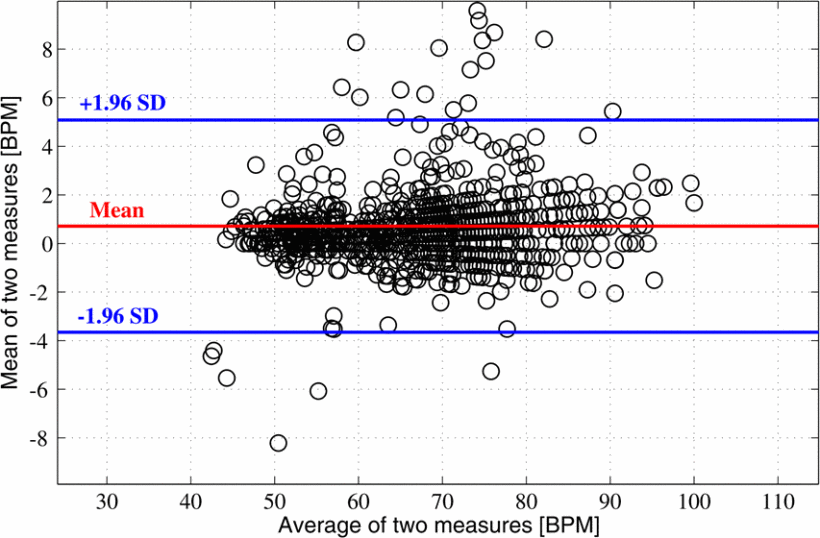
\includegraphics[width=0.7\textwidth]{pic/bland-altman-pino.png}
		\caption[Bland-Altman Graph zwischen von \ac{EKG} und \ac{BKG} berechneter \ac{HR}]{Bland-Altman Graph zwischen von \ac{EKG} und \ac{BKG} berechneter \ac{HR}}
		\label{fig:bland-altman-pino}
	\end{figure}
	
	Hier zeigt sich, dass beim Großteil des hier betrachteten Signals die \ac{HR} größtenteils mit einer Genauigkeit von $\pm$ Schläge pro Minute bestimmt werden konnte. Allerdings handelt es sich hier um im Sitzen aufgenommenes Signal, bei dem die Variabilität geringer ist als bei in Betten aufgenommenem \ac{BKG}.
	
	
	\subsection{Maschinelles Lernen mit statistischen Merkmalen}
	
	Ein Algorithmus zur Beurteilung der Signalqualität mittels maschinellen Lernens wird von \citeauthor{Sadek2016} im Paper \citetitle{Sadek2016} beschrieben. Betrachtet werden \ac{BKG}-Signale, die in einem Massagesessel aufgenommen werden, also ebenfalls im Sitzen aufgenommenes Signal, bei dem eine geringere Variabilität als in unserem Anwendungsfall erwartet wird.
	
	Die vorliegenden Daten wurden manuell von Expert*innen als informativ oder nicht informativ klassifiziert und in 10-Sekunden-Segmente, die sich nicht überlappen, aufgeteilt, die sich nicht überlappen. Insgesamt waren 58 \% der Daten als informativ und 42 \% als nicht-informativ gelabelt. Von diesen Segmenten wurden nach einer Bandpass-Filterung auf 1 bis 12 Hz 13 statistische Merkmale berechnet:
	\begin{itemize}
		\item Minimun
		\item Maximum
		\item Mittelwert
		\item Standardabweichung
		\item Schiefe
		\item Kurtosis
		\item Spannweite
		\item Interquartilspannweite
		\item mittlere absolute Abweichung
		\item Anzahl der Nulldurchgänge
		\item Varianz der lokalen Minima
		\item Varianz der lokalen Maxima
		\item Mittelwerte der Signalhüllkurve\footnote{Die Signalhüllkurve ist eine glatte Kurve, die die Extrema des Signals umreißt.}
	\end{itemize}
	
	Für fünf verschiedene Modelle des maschinellen Lernens wurden jeweils die besten Hyperparameter über Kreuzvalidierung auf den Trainingsdaten ermittelt und die Modelle anschließend mit diesen Hyperparametern trainiert. Anschließend wurden die Modelle auf unbekannten Daten getestet. Das Training und Testen wurde mit getauschten Gruppen wiederholt. Das beste Ergebnis wurde mit einem Random Forest erreicht: Die durchschnittliche Genauigkeit der Kreuzvalidierung betrug 98,13 \% bzw. 100 \% bei getauschten Gruppen. Auf dem Testset wurde eine Genauigkeit von 92,3 \% bzw. 97,99 \% erreicht. Weitere Evaluationsmetriken außer eine \textit{Confusion Matrix} für den besten Klassifkator sind nicht gegeben.
	
	Diese Ergebnisse sind sehr gut, allerdings muss bei der Einordnung beachtet werden, dass bei für die Kreuzvalidierung die Segmente zufällig verteilt wurden und nicht beachtet wurde, dass der Algorithmus für aussagekräftige Validierung einzelne Personen nicht darf. Dadurch ist die Performance auf gänzlich unbekannten Daten weiterhin nicht bekannt und vermutlich schlechter, als die Zahlen es hier vermuten lassen.
	
	\subsection{Ähnlichkeit der Intervallschätzer des CLIE-Algorithmus}
	
	Ein weiteres Maß für die Signalqualität basiert auf dem in \ref{CLIE} vorgestellten Algorithmus zur Intervallschätzung. Dieser \acl{SQI} misst, wie einig sich die drei Intervallschätzer sich. Wenn diese sich uneinig sind, ist der \ac{SQI} bei 0, je ähnlicher sich die Schätzungen sind, desto höher ist er. Für jedes Fenster $i$ wird er wie folgt berechnet: \[ q = \frac{E_f[n_{opt}, i]}{\sum E_f[n, i]} \]
	

\section{Messdaten}
	
	\subsection{Erfassung}
	
	\begin{itemize}
		\item aufgenommen in der Gefäßstation des Universitätskrankenhauses in Tampere in Finnland
		\item 14 Patient*innen wurden bis zu 24 h überwacht
		\item 2 weiblich, 12 männlich
		\item Durchschnittsalter: 69,57 Jahre
		\item nach verschiedenen gefäßchirurgischen Eingriffen
		\item durchschnittliche Messdauer: 17.7 h, range 4,46 bis 22,96 h
		\item EMFit QS Bettsensor, zwischen Matratze des Krankenhausbettes und Bettgestehl positioniert
		\item Samplingrate des EMFit QS Systems: 100 Hz, Bandpass-limitiert auf 1 bis 5 Hz
		\item Referenz EKG: Faros 360 5 lead Holter monitor, 1 kHz Abtastrate
		\item variabler Drift zwischen beiden Signalen % TODO: näher beschreiben
	\end{itemize}
	
	\subsection{Vorliegende Form}
	
	\begin{itemize}
		\item unbearbeitetes \ac{BKG}-Signal, abgesehen von der Bandpasslimitierung auf 1 bis 5 Hz
		\item unbearbeitetes 3-Kanal EKG Signal
		\item mit CLIE-Algorithmus detektierte Herzschläge, schon nach Qualität gefiltert mitsamt Brüser SQI, Länge und Länge des Herzschlages der EKG Referenz
		\item Vektoren, die den Drift der beiden Signale beschreiben, Form Sekunde \ac{BKG}-Signal und entsprechende Sekunde in \ac{EKG}-Referenz
	\end{itemize}
	
	\subsection{Verarbeitung und Datenstruktur}
	
	\begin{itemize}
		\item Datensatz von einem Patient besteht aus BKG Signal und EKG Referenz
		\item beides wird eingelesen, geprüft ob schon Detektion von Herzschlägen (Erkennen von R-Peaks bzw. CLIE Algorithmus schon durchgeführt wurde und als csv-Datei existiert
	\end{itemize}

	\subsection{Annotation der Daten}
	
	Die vorliegenden Daten sind nicht annotiert. Es ist im Rahmen dieser Arbeit nicht möglich, die Annotation durch Expert*innen durchführen zu lassen, weshalb auf das parallel aufgenommene \ac{EKG} zurückgegriffen wird.
	
	\begin{itemize}
		\item aufgrund des nicht-linearen Drifts der Daten herzschlaggenaue Synchronisierung schwierig
		\item Entscheidung Annotation von Bereichen von mehren Sekunden möglich zu machen
		\item Ablauf: existiert EKG Signal zu diesem Zeitpunkt, bei dem eine Herzfrequenz ermittelt werden konnte
		\item Berechnung dieser -> Anzahl der R-Peaks in diesem Bereich -1 geteilt durch den Abstand des letzten und des ersten Peaks
		\item Berechnung \ac{BKG}-Herzfrequenz: Durchschnitt der geschätzten Längen der erkannten Peaks im Bereich
		\item Annotation anhand von relativer oder absoluter Abweichung der beiden
	\end{itemize}
	


\chapter{Analyse}\label{analyse}

In diesem Kapitel werden die vorgestellten Daten näher untersucht. Das beinhaltet sowohl die Anwendung der in Kapitel\,\ref{artefakterkennung} beschriebenen existierenden Verfahren als auch eine Analyse der verwendeten Merkmale.

\section{Aufbau und Evaluation der Verfahren}

Um Modelle zur Beurteilung der Signalqualität anzuwenden und zu untersuchen, müssen sowohl die verwendeten Merkmale extrahiert als auch die Ergebnisse evaluiert werden. In den hier durchgeführten Untersuchungen wurde die Segmentlänge standardmäßig auf 10\,Sekunden festgelegt und der Abstand der Segmente auf 1\,Sekunde, wodurch sich die Segmente zu je 90\,\% überlappen. Diese Segmentlänge wird zum einen häufig verwendet\footcite[Vgl.][]{Yu2020, Sadek2016, Orphanidou2015}, zum anderen bietet sie eine ausreichend große Robustheit für die Annotation der Daten. Die für die Verfahren jeweils benötigten Merkmale werden segmentweise extrahiert und serialisiert. Zusätzlich zu den verwendeten Merkmalen werden allgemeine Informationen über die Segmente gespeichert. Dazu gehören Patient*innen-ID, EKG-Herzrate, BKG-Herzrate, absoluter und relativer Fehler, $E\textsubscript{HR}$ und die binäre Annotation. Für letztere wird als Standard $E\textsubscript{HR} = 10$ als Schwellwert verwendet.

Diese Daten werden anschließend in Trainings- und Testset aufgeteilt. Um diese beiden Gruppen inhaltlich vollständig zu trennen und auszuschließen, dass auf teilweise bekannten Daten validiert wird, geschieht die Trennung anhand der Patient*innen-IDs, sodass Segmente einer Person lediglich in einem der beiden Sets verwendet werden. Das Testset in dieser Arbeit entspricht einem Drittel der Patient*innen, die restlichen zwei Drittel werden zur Datenexploration, zur Merkmalskonstruktion und zum Training verwendet. Die Verteilung von $E\textsubscript{HR}$ im Testset ist in Abbildung\,\ref{fig:validation-set} gezeigt. Von den existierenden Verfahren benötigen zwei keine Trainingsphase; um vergleichbare Ergebnisse zu erhalten, wird auch bei diesen bei der Evaluation nur das Testset betrachtet.

\begin{figure}[h]
	\centering
	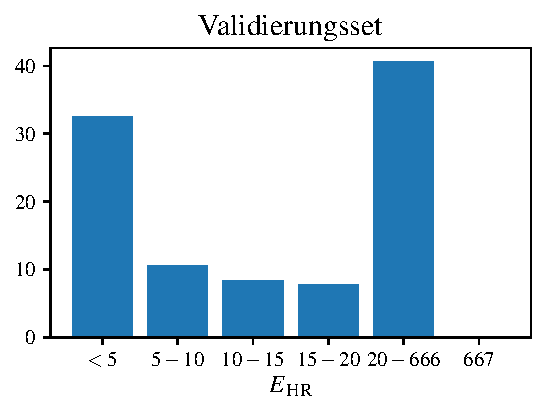
\includegraphics{pic/mlp-statistical-testset.pdf}
	\caption[Verteilung von $E\textsubscript{HR}$ auf dem Testset.]{Verteilung von $E\textsubscript{HR}$ auf dem Testset, wobei 667\,\si{FE} dem maximalen Fehler entspricht.}
	\label{fig:validation-set}
\end{figure}


Wie schon in Kapitel\,\ref{artefakterkennung} beschrieben, sind bei der Verarbeitung von medizinischen Signalen zwei Kenngrößen wichtig: Die Coverage und die Qualität des Signals, in diesem Fall also die Genauigkeit der geschätzten Herzrate im Vergleich zur Referenz. Diese beiden müssen gegeneinander aufgewogen werden und werden aus diesem Grund beide betrachtet. Die Qualität der Modelle kann zunächst anhand der binären Klassifikation beurteilt werden. Da diese aber keine Auskunft darüber enthält, wie nah ein klassifiziertes Signal an dem Schwellwert für $E\textsubscript{HR}$ liegt, wird das in einer tiefergehenden Evaluation ebenfalls betrachtet. Insbesondere falsch klassifiziertes Signal, also Falsch-Negative und Falsch-Positive, ist interessant, um zu beurteilen, ob Fehlklassifikationen lediglich im Grenzbereich $E\textsubscript{HR} \approx 10$\,\si{FE} oder allgemein vorkommen. Im Zuge der tiefergehenden Evaluation wird sowohl der Fehler auf dem als informativ klassifizierten Signal betrachtet als auch die Coverage in Bezug auf das ganze Signal für verschiedene Fehlergrößen.

\section{Anwendung existierender Verfahren}

Zunächst werden die in Kapitel\,\ref{artefakterkennung} beschriebenen existierenden Artefakterkennungsverfahren mit den in dieser Arbeit untersuchten Daten wie oben beschrieben getestet und ihre Leistungsfähigkeit untersucht und bewertet.

\subsection{Ähnlichkeit der Intervallschätzer des CLIE-Algorithmus}\label{eval-brueser}

Der \ac{SQI}, der die Ähnlichkeit der Intervallschätzer des \ac{CLIE}-Algorithmus angibt, wird im Normalfall herzschlagweise angewendet. Da die Datenannotion nur bereichsweise vorgenommen werden kann, wurde entschieden, ein Segment als informativ zu klassifizieren, wenn mit den Herzschlägen, deren \ac{SQI} über einem Schwellwert $q_{th}$ liegt, eine Coverage über einem gegebenen Schwellwert $c_{th}$ auf dem Segment erreicht wird. Getestete Schwellwerte für die Coverage sind 50\,\%, 75\,\% und 100\,\%. Zum Testen des Algorithmus wurde unter anderem $q_{th} = 0{,}4$ gewählt, da dieser Wert auch von \citeauthor{Zink2017} verwendet wird.\footcite[]{Zink2017} Zusätzlich wurden $q_{th} = 0{,}3$ und $q_{th} = 0{,}2$ untersucht, um den Einfluss von $q_{th}$ einzuordnen. Bei der Berechnung der Merkmale werden für jedes Segment die detektierten Herzschläge extrahiert, deren \ac{SQI} über $q_{th}$ liegt. Auf Basis dieser Intervalllängen wird wie in Kapitel\,\ref{annotation} beschrieben die Herzrate, im Folgenden $HR\textsubscript{SQI}$ genannt, ermittelt. Extrahierte Merkmale sind damit in diesem Fall $HR\textsubscript{SQI}$ und die Coverage $C\textsubscript{SQI}$. Für die Auswertung muss beachtet werden, dass sich die ermittelte Herzrate $HR\textsubscript{SQI}$ von der zur Annotation verwendeten Herzrate unterscheiden kann. Aufgrund der Vergleichbarkeit wird $HR\textsubscript{SQI}$ nicht für die Berechnung des \ac{MAE} des Algorithmus verwendet.

Bei einer ersten Betrachtung von \ac{MAE} in \si{FE}, Coverage und Accuracy wird sichtbar, dass die Wahl der Schwellwerte großen Einfluss auf das Ergebnis hat und in jedem Fall Aussagekraft des Signals gegen Coverage eingetauscht wird. Die genauen Ergebnisse sind in Tabelle\,\ref{fig:brueser-sqi-MAE-Coverage} zu finden. Auch ist deutlich, dass die Accuracy der Klassifikation mit mit Werten knapp über 0{,}6 nicht gut ist. Des Weiteren ist die Coverage bei verhältnismäßig kleineren \ac{MAE} sehr niedrig.
 
  \begin{table}[h]
  
 	\centering
 	\begin{tabular}{l || c | c | c}
 									& \ac{MAE} [\,\si{FE}]	& Coverage [	\%]	& Accuracy\\ \hline
 		insgesamt 					& 21{,}85				& -				& - \\
 		annotiert					& 3{,}28					& 43{,}22		& - \\ \hline
 		$q_{th}=0{,}4, c_{th}=50$	& 12{,}30				& 20{,}95		& 0{,}65\\
 		$q_{th}=0{,}4, c_{th}=75$	& 9{,}57					& 11{,}78		& 0{,}63\\
 		$q_{th}=0{,}4, c_{th}=100$	& 8{,}77					& 5{,}26			& 0{,}60\\ \hline
 		$q_{th}=0{,}3, c_{th}=50$	& 21{,}36				& 58{,}73		& 0{,}55\\
 		$q_{th}=0{,}3, c_{th}=75$	& 17{,}97				& 37{,}87		& 0{,}62\\
 		$q_{th}=0{,}3, c_{th}=100$	& 13{,}45				& 19{,}25		& 0{,}63\\ \hline
 		$q_{th}=0{,}2, c_{th}=75$	& 21{,}39				& 96{,}43		& 0{,}44\\
 	\end{tabular}
 	\caption[Fehler und Coverage der Klassifikation nach der Ähnlichkeit der Intervallschätzer des CLIE-Algorithmus für verschiedene Schwellwerte im Vergleich zum gesamten Signal und der Annotation.]{Fehler und Coverage für verschiedene Schwellwerte im Vergleich zum gesamten Signal und der Annotation.}
 	\label{fig:brueser-sqi-MAE-Coverage}
 	\end{table}
 	
 Die detailliertere Evaluation wird beispielhaft für die Schwellwerte $q_{th} = 0.4$ und $q_{th} = 0.3$ mit $c_{th}=75$ vorgestellt. Positiv hervorzuheben ist, dass bei beiden kein Signal als informativ klassifiziert wird, bei denen $E\textsubscript{HR}$ maximal ist. Allerdings ist bei über 20\,\% der mit $q_{th} = 0.4$ als informativ klassifizierten Segmenten $E\textsubscript{HR}$ größer als 20, mit $q_{th} = 0.3$ bei sogar mehr als 35\,\%, wie auch in Abbildung\,\ref{fig:brueser-positives} abgebildet. Das bedeutet, dass Falschklassifikationen nicht nur im Randbereich vorkommen. Dies wird noch deutlicher, wenn man sich den \ac{MAE} auf jeweils auf den Falsch-Positiven und Falsch-Negativen anschaut. So beträgt der \ac{MAE} bei $q_{th} = 0.4$ für falsch-negative Segmente 3,65\,\si{FE}, ist also nah an dem \ac{MAE} aller informativen Segmente von 3,28\,\si{FE}. 
 
 \begin{figure}[H]
 	\centering
		\begin{subfigure}{.45\textwidth}
			\centering
 			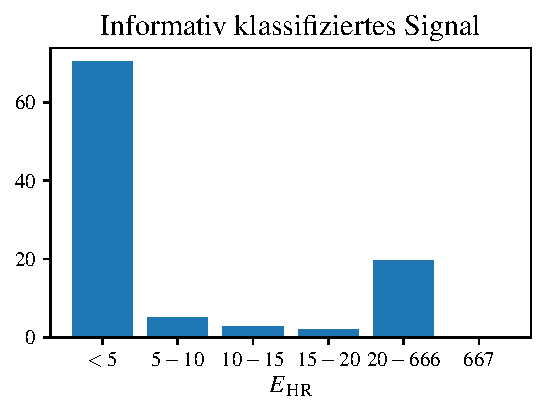
\includegraphics[scale=0.7]{pic/brueser04-positives.pdf}
 			\caption[$q_{th}=0.4$]{$q_{th}=0.4$}
 		\end{subfigure}
    	\begin{subfigure}{.45\textwidth}
    		\centering
 			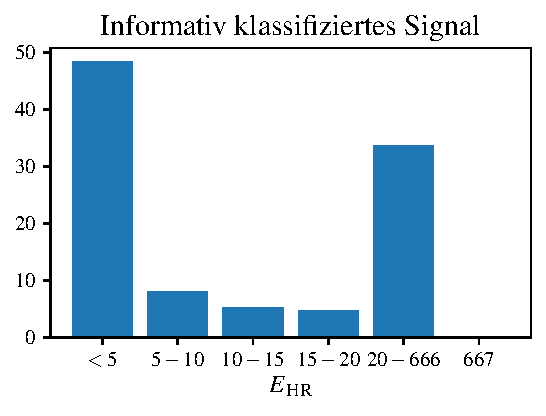
\includegraphics[scale=0.7]{pic/brueser03-positives.pdf}
 			\caption[$q_{th}=0.3$]{$q_{th}=0.3$}
 		\end{subfigure}
 	\caption[Verteilung von $E\textsubscript{HR}$ bei den als informativ klassifizierten Segmenten durch Betrachtung der Ähnlichkeit der \ac{CLIE}-Intervallschätzer.]{Verteilung von $E\textsubscript{HR}$ bei den als informativ klassifizierten Segmenten.}
 	\label{fig:brueser-positives}
 \end{figure}
 
 Außerdem wurde untersucht, wie hoch die Coverage unter einem bestimmten Fehler $E\textsubscript{HR}$ auf dem gesamten Signal ist, wenn nur die als informativ klassifizierten Segmente verwendet werden. Hier wird besonders sichtbar, wie niedrig die erreichte Coverage ist. So werden mit $q_{th}=0{,}4$ und $c_{th}=75$ nur 8{,}29\,\% Coverage für $E\textsubscript{HR} < 5$ erreicht werden, obwohl das ganze Signal 32{,}61\,\% enthält. Mit $q_{th}=0{,}3$ und $c_{th}=75$ sind es immerhin 18{,}32\,\%, aber auch das liegt deutlich unter dem tatsächlichen Wert. Die Verteilung ist in Tabelle\,\ref{fig:brueser-coverage} gezeigt.
 
 \begin{table}[h]
 	\centering
  	\begin{tabular}{l || c | c | c}
 											& insgesamt 		& $q_{th}=0{,}3, c_{th}=75$ & $q_{th}=0{,}4, c_{th}=75$\\\hline
 		$E\textsubscript{HR} < 5$\,\si{FE} 	&  32{,}61\,\% 	& 18,32\,\% 					& 8,29\,\%	\\
 		$E\textsubscript{HR} < 10$\,\si{FE} 	&  43{,}21\,\% 	& 21,34\,\% 					& 8,89\,\%	\\
 		$E\textsubscript{HR} < 15$\,\si{FE} 	&  51{,}64\,\% 	& 23,35\,\% 					& 9,22\,\%	\\
 		$E\textsubscript{HR} < 20$\,\si{FE} 	&  59{,}38\,\% 	& 25,12\,\% 					& 9,47\,\%\\
 	\end{tabular}
 	\caption[Coverage unter bestimmten Fehlern $E\textsubscript{HR}$ vor und nach Klassifikation durch Betrachtung der Ähnlichkeit der \ac{CLIE}-Intervallschätzer.]{Coverage unter bestimmten Fehlern $E\textsubscript{HR}$ vor und nach Klassifikation.}
 	\label{fig:brueser-coverage}
 \end{table}
 
 Alles in allem zeigt sich, dass trotz einer sehr niedrigen erreichten Coverage der Fehler in der Klassifikation verhältnismäßig hoch ist. Wenn $q_{th}$ und $c_{th}$ nicht zu niedrig gewählt werden, kann ein Teil des nicht informativen Signals markiert und somit der Fehler in weiterer Verarbeitung insgesamt reduziert werden. 
 

\subsection{Schwellwertbasierte Artefakterkennung}

Für das zweite getestete Verfahren werden lediglich zwei Schwellwerte $T_1$ und $T_2$ benötigt, die auf Standardabweichung, Minimum, Maximum und Durchschnitt des Signals beruhen. Die Klassifikation ist ein einfacher Vergleich. \citeauthor{Pino2015} verwenden sehr kleine Fenster, die hier aufgrund fehlender Robustheit der Annotation nicht verwendet werden können.\footcite[]{Pino2015} Stattdessen wird der Algorithmus sowohl auf 10\,Sekunden- als auch 4\,Sekunden-Segmenten getestet, um schlechte Ergebnisse bedingt durch eine bestimmte Segmentlänge auszuschließen.

Die Tests mit beiden Segmentlängen zeigen, dass dieses Verfahren für die in dieser Arbeit untersuchten Daten nicht nutzbar ist, da bei beiden über 95\,\% der Daten als informativ klassifiziert werden, darunter auch Segmente, bei denen $E\textsubscript{HR}$ maximal ist. Weiterführende Evaluation bietet hier keine weiteren Erkenntnisse. Dieses Verfahren ist damit nicht weiter nutzbar.

\subsection{Maschinelles Lernen mittels statistischer Merkmale}\label{res-statistical}

Für das maschinelle Lernen mittels statistischer Merkmale werden die in Kapitel\,\ref{ml-beschreibung} aufgezählten Merkmale extrahiert. Als Bibliothek für die Modelle des maschinellen Lernens wird \textit{scikit-learn}\footcite[]{scikit-learn} verwendet. Da die Daten sich grundlegend von den von \citeauthor{Sadek2016} untersuchten unterscheiden, werden die Hyperparameter der Modelle im Zuge dieser Arbeit erneut optimiert. Bei der dafür durchgeführten Kreuzvalidierung wird wie schon bei der Unterteilung in Trainings- und Testset anhand der Patient*innen-ID geteilt, damit auch diese aussagekräftige Ergebnisse liefert.

Insgesamt zeigen bereits Accuracy und \ac{MAE}, siehe Tabelle\,\ref{fig:ml-statistical-MAE-Coverage}, eindeutig, dass die Klassifikation von keinem der Modelle den Ergebnissen des Papers von \citeauthor{Sadek2016}\footcite{Sadek2016} entspricht. Die Accuracy und AUC von je unter 0,6 zeigen, dass die Klassifikation nur minimal besser als reines Raten ist. Teils ist der \ac{MAE} der als informativ klassifizierten Segmente sogar größer als der auf dem gesamten Signal. In der folgenden tiefergehenden Evaluation werden lediglich \ac{RF} und \ac{MLP} betrachtet. Zwar sind die Ergebnisse des \ac{DT} auf einem ähnlichen Niveau, aber da ein \ac{RF} lediglich ein Zusammenschluss mehrerer \ac{DT} ist, ist eine zusätzliche Analyse nicht lohnenswert. 

\begin{table}[H]
	\centering
 	\begin{tabular}{l || c | c | c | c | c}
 					& \makecell{\ac{MAE}\\{[\,\si{FE}]}}	& \makecell{Coverage\\{[\,\%]}}	& \makecell{Accuracy\\(Testset)}	& \makecell{Accuracy\\(Kreuzvalidierung Trainingsset)}	& AUC\\ \hline
 		insgesamt 	& 21{,}84				& -				& - 									& -														& -\\
 		annotiert	& 3{,}28					& 43{,}22\,\%	& - 									& -														& -\\ \hline
 		\acs{LDA}	& 21{,}84				& 84{,}81\,\%	& 0{,}49								& 0{,}51												& 0,53\\
 		\acs{SVM}	& 22{,}06				& 88{,}14\,\%	& 0{,}47								& 0{,}55												& 0,53\\
 		\acs{DT}	& 19{,}47				& 70{,}39\,\%	& 0{,}55								& 0{,}55												& 0,59\\
 		\acs{RF}	& 20{,}14				& 62{,}02\,\%	& 0{,}55								& 0{,}58												& 0,59\\
 		\acs{MLP}	& 18{,}41				& 42{,}04\,\%	& 0{,}56								& 0{,}54												& 0,58\\
 	\end{tabular}
 	\caption[Fehler und Coverage der Klassifikation für die verschiedenen Modellen des maschinellen Lernens mit statistischen Merkmalen im Vergleich zum gesamten Signal und der Annotation.]{Fehler und Coverage für die verschiedenen Modelle im Vergleich zum gesamten Signal und der Annotation.}
 	\label{fig:ml-statistical-MAE-Coverage}
\end{table}

Bei einer ähnlich hohen, beziehungsweise höheren Coverage als die der Annotation ist der deutlich höhere \ac{MAE} der Klassifikation in falsch-positiven Segmenten begründet. Der Anteil von Segmenten mit einem Fehler $E\textsubscript{HR}$ größer als 20\,\si{FE} ist bei beiden Modellen mit 35 bis 40\,\% ähnlich hoch. Zusätzlich sind 0{,}002\,\% der vom \ac{RF} als informativ klassifizierten Segmente solche, bei den $E\textsubscript{HR}$ maximal ist. Das bedeutet, dass die falsch-positiv klassifizierten Segmente bei beiden Klassifikatoren keine Randfälle sind. Der \ac{MAE} der falsch-negativen Klassifikationen beträgt beim \ac{RF} 4,07\,\si{FE} und beim \ac{MLP} 3{,}39\,\si{FE}, ist also leicht höher als der \ac{MAE} aller informativen Segmente, aber nicht relevant. Auch bei diesen handelt es sich demnach nicht um Randfälle.
 	
 \begin{figure}[H]
 	\centering
		\begin{subfigure}{.45\textwidth}
			\centering
 			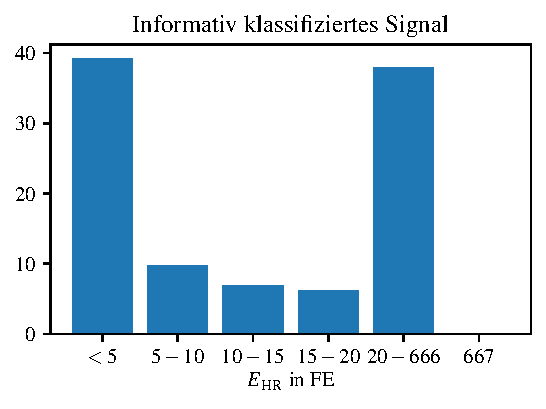
\includegraphics[scale=0.7]{pic/rf-statistical-positives.pdf}
 			\caption[RF]{RF}
 		\end{subfigure}
    	\begin{subfigure}{.45\textwidth}
    		\centering
 			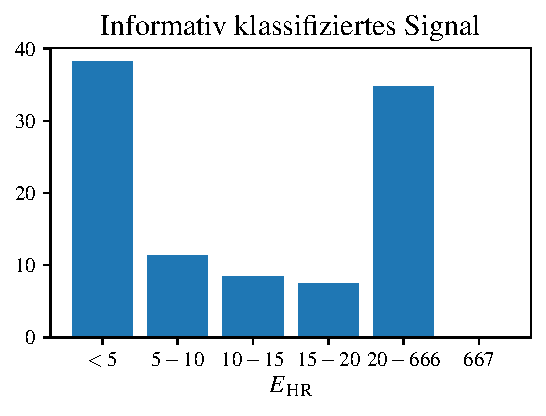
\includegraphics[scale=0.7]{pic/mlp-statistical-positives.pdf}
 			\caption[MLP]{MLP}
 		\end{subfigure}
 	\caption[Verteilung von $E\textsubscript{HR}$ bei den als informativ klassifizierten Segmenten nach Klassifikation mittels statistischen Merkmalen.]{Verteilung von $E\textsubscript{HR}$ bei den als informativ klassifizierten Segmenten.}
 	\label{fig:ml-statistical-positives}
 \end{figure}
 
 Auch für diese Modelle wird untersucht, wie hoch die Coverage unter einem bestimmten Fehler $E\textsubscript{HR}$ bei der Betrachtung des als informativ klassifizierten Signals auf dem ganzen Signal ist. Auffallend ist, dass die Werte beim \ac{MLP} knapp halb so hoch wie die tatsächliche Coverage sind. Das zeigt ergänzend zu der gemessen Accuracy, dass ca. die Hälfte der Segmente, unabhängig von ihrer tatsächlichen Qualität, als informativ klassifiziert werden. Der \ac{RF} ist näher an der tatsächlichen Coverage, aber es wird auch mehr nicht-informatives Signal falsch-positiv klassifiziert. Die Werte sind in Tabelle\,\ref{fig:ml-statistical-coverage} aufgelistet.
 
  \begin{table}[H]
 	\centering
  	\begin{tabular}{l || c | c | c}
 											& insgesamt 		& RF			& MLP\\\hline
 		$E\textsubscript{HR} < 5$\,\si{FE} 	&  32{,}61\,\% 	& 24,34\,\%	& 16,07\,\%	\\
 		$E\textsubscript{HR} < 10$\,\si{FE} 	&  43{,}22\,\% 	& 30,35\,\% 	& 20,82\,\%	\\
 		$E\textsubscript{HR} < 15$\,\si{FE} 	&  51{,}66\,\% 	& 34,66\,\% 	& 24,34\,\%	\\
 		$E\textsubscript{HR} < 20$\,\si{FE} 	&  59{,}40\,\% 	& 38,52\,\% 	& 27,45\,\%\\
 	\end{tabular}
 	\caption[Coverage unter bestimmten Fehlern $E\textsubscript{HR}$ vor und nach Klassifikation mittels statistischen Merkmalen.]{Coverage unter bestimmten Fehlern $E\textsubscript{HR}$ vor und nach Klassifikation.}
 	\label{fig:ml-statistical-coverage}
 \end{table}
 
 Insgesamt zeigt sich, dass die Klassifikation mittels statistischer Merkmale bei vorliegenden Daten und Annotation nicht sehr zuverlässig ist. Zwar wurden auf anderen Daten sehr gute Ergebnisse erreicht, aber es bestätigt sich die Vermutung, dass sich dies, vermutlich aufgrund der unterschiedlichen Aufnahmesituation der Daten und der nicht aussagekräftigen Validierung der Ergebnisse für die im Paper untersuchten Daten, nicht übertragen lässt. 
 
\section{Analyse der Merkmale}

Obwohl keines der Verfahren sehr gute Ergebnisse für die vorliegenden Daten liefert, ist besonders bei den Modellen maschinellen Lernens interessant, welchen Einfluss und welchen Informationsgewinn die jeweiligen Merkmale haben. Aus diesem Grund wird im Folgenden eine explorative Datenanalyse durchgeführt.

Zunächst wird betrachtet, ob die Merkmale untereinander und mit $E\textsubscript{HR}$ und der Annotation korreliert sind. Da die Merkmale das Segment gemeinschaftlich statistisch beschreiben, ist eine hohe Korrelation untereinander erwartet und zeigt sich auch. Eine Ausnahme bilden Kurtosis, Mittelwert und Schiefe. Die Anzahl der Nulldurchgänge ist ebenfalls nur schwächer mit den restlichen Mermalen korreliert. Außerdem zeigt sich bei der Betrachtung des in Abbildung\,\ref{fig:corr-heatmap-statistical} abgebildeten Korrelationsdiagramms, dass die Korrelation zu $E\textsubscript{HR}$ und der Annotation nicht signifikant ist. Auch bei paarweiser Visualisierung zeigt sich, dass sich anhand keines untersuchten Merkmalspaares informative von nicht informativen Segmenten unterscheiden lassen.

\begin{figure}[H]
	\centering
	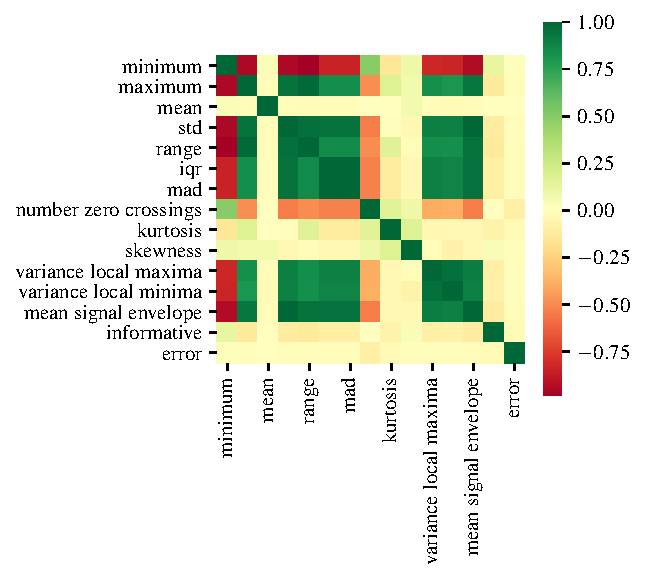
\includegraphics[scale=0.95]{pic/corr-heatmap-statistical.pdf}
	\caption{Korrelationsdiagramm der statistischen Merkmale, $E\textsubscript{HR}$ und der binären Annotation.}
	\label{fig:corr-heatmap-statistical}
\end{figure}

Weiteren Einblick ermöglicht die Analyse des \ac{RF}, da bei diesem ermittelt werden kann, wie wichtig die einzelnen Merkmale jeweils für die Entscheidungsfindung sind. Das Ergebnis zeigt, dass der Durchschnitt des Signals deutlich weniger Einfluss als die anderen betrachteten Merkmale hat. Die Schiefe (skewness) und die Anzahl der Nulldurchgänge sind, wie in Abbildung\,\ref{fig:rf-statistical-importances} sichtbar, die beiden wichtigsten Merkmale. 

\begin{figure}[H]
	\centering
	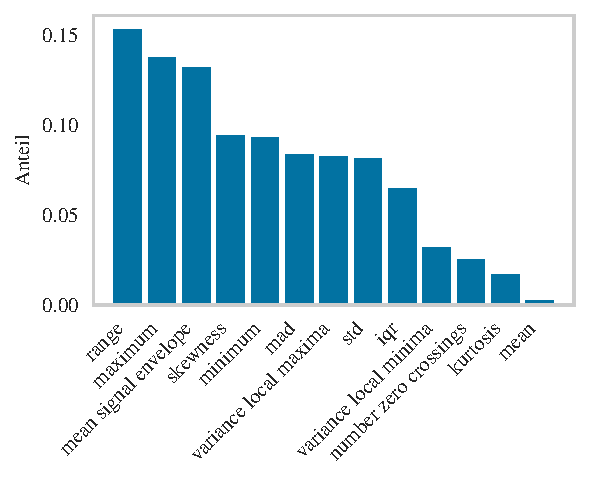
\includegraphics[scale=0.95]{pic/rf-cl-statistical.pdf}
	\caption{Wichtigkeit der Merkmale für den \ac{RF}-Klassifikator mit statistischen Merkmalen.}
	\label{fig:rf-statistical-importances}
\end{figure}

Da die Visualisierung hochdimensionaler Daten schwierig ist und auch Modelle maschinellen Lernens bei einer hohen Merkmalszahl aufwändiger zu trainieren sind, wurde ebenfalls untersucht, wie sich die Daten bei einer Transformation in einen niedriger dimensionierten Raum verhalten. Untersuchte Transformationen umfassen sowohl unüberwachte Verfahren wie eine \ac{PCA} mit verschiedenen Kerneln als auch überwachte Verfahren wie eine Dimensionsreduktion mit einer \ac{LDA}. Auch die transformierten Daten lassen sich nicht voneinander trennen, wie auch in Abbildung\,\ref{fig:dim-red-statistical} beispielhaft für eine \ac{PCA} mit linearem Kernel gezeigt ist.


 \begin{figure}[H]
 	\centering
 	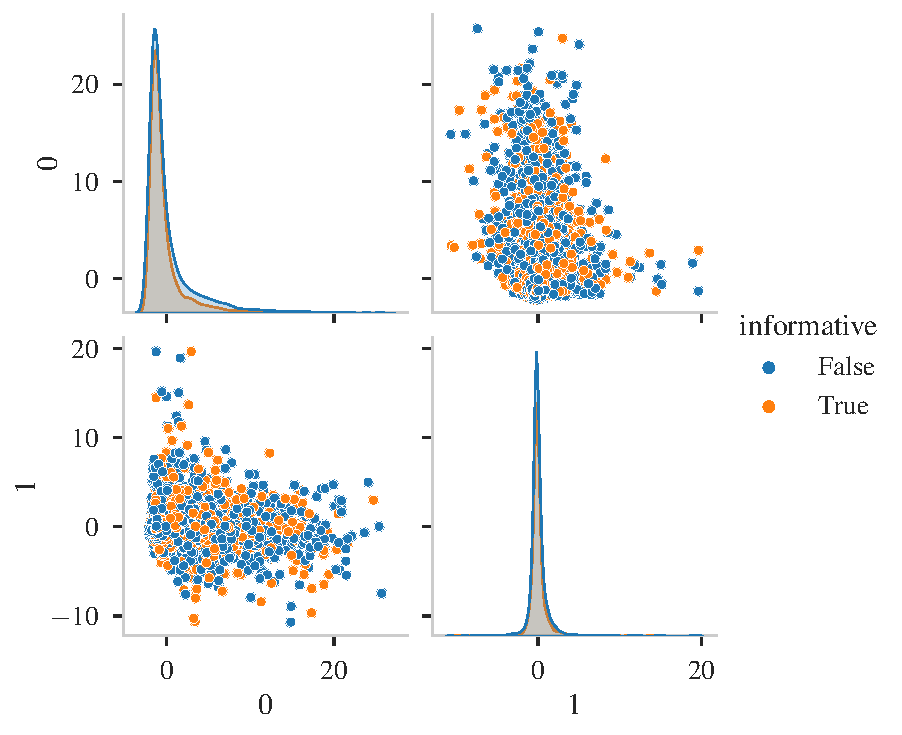
\includegraphics[width=0.6\textwidth]{pic/statistical-pca-lin.pdf}
	\caption{Dimensionsreduktion der statistischen Merkmale mit einer \ac{PCA} mit linearem Kernel.}
	\label{fig:dim-red-statistical}
\end{figure}

Da eine hohe Korrelation zwischen einzelnen Merkmalen, wie sie auch bei den statistischen Merkmalen vorliegt, dazu führen kann, dass die Interpretation der Wichtigkeit der Merkmale und die Qualität der Modelle generell eingeschränkt ist\footcite[Kapitel 8]{Harrison2019}, wird außerdem die Abhängigkeit der Merkmale voneinander untersucht. Hierzu wird das Python-Paket \texttt{rfimp} verwendet, das ermittelt, welche Merkmale durch andere vorhergesagt werden können. Nach Reduktion der Merkmalsmenge um diese bleiben lediglich fünf Merkmale: die Standardabweichung, der Durchschnitt, die Anzahl der Nulldurchgänge, Schiefe und Kurtosis. Betrachtet man für diese die Wichtigkeit der einzelnen Merkmale bei einem \acl{RF}, zeigt sich, dass weiterhin der Durchschnitt am wenigsten Einfluss besitzt, wobei die Standardabweichung jetzt am wichtigsten ist. Die gesamte Verteilung ist in Abbildung\,\ref{fig:rf-statistical-reduced} sichtbar.

\begin{figure}[H]
	\centering
	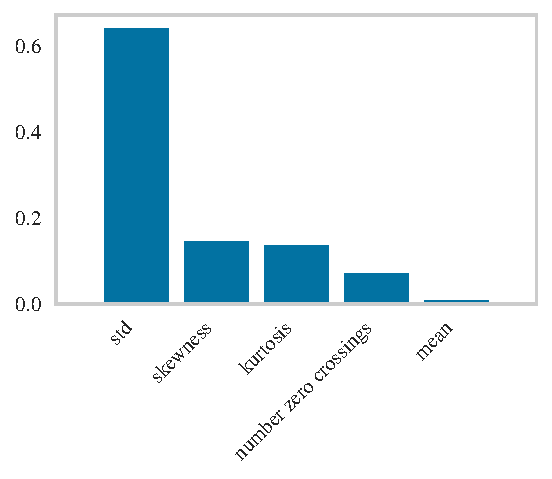
\includegraphics[scale=0.85]{pic/rf-reduced-statistical.pdf}
	\caption{Wichtigkeit der Merkmale für den \ac{RF}-Klassifikator mit reduziertem Merkmalsset statistischer Merkmale.}
	\label{fig:rf-statistical-reduced}
\end{figure}

Die Ergebnisse dieses \acl{RF}s mit reduzierter Merkmalsanzahl können mit dem in Kapitel\,\ref{res-statistical} untersuchten \acl{RF} verglichen werden. Der \ac{MAE} und die Coverage sind bei reduzierter Merkmalszahl geringfügig niedriger, die AUC deutlich. Insgesamt sind die Klassifikatoren auf einem ähnlichen Niveau, auch wenn dieser Vergleich bei der geringen Qualität schwierig ist. In Tabelle\,\ref{fig:ml-statistical-reduced-comparison} sind die beiden \acl{RF}s gegenübergestellt.

 \begin{table}[H]
 	\centering
  	\begin{tabular}{l || c | c | c}
 																& insgesamt 		& RF mit 13 Merkmalen			& RF mit 5 Merkmalen\\\hline
 		$E\textsubscript{HR} < 5$\,\si{FE} 						& 32{,}61\,\% 		& 24,34\,\%			& 23,43\,\%	\\
 		$E\textsubscript{HR} < 10$\,\si{FE} 						& 43{,}22\,\% 		& 30,35\,\% 		& 28,98\,\%	\\
 		$E\textsubscript{HR} < 15$\,\si{FE} 						& 51{,}66\,\% 		& 34,66\,\% 		& 32,94\,\%	\\
 		$E\textsubscript{HR} < 20$ \,\si{FE}						& 59{,}40\,\% 		& 38,52\,\% 		& 36,45\,\%\\\hline
 		MAE														& 21{,}85\,\si{FE}	& 20,14\,\si{FE}	& 19{,}48\,\si{FE}\\\hline
 		Coverage												& 43{,22}\,\%		& 62,02\,\%			& 57,58\,\%\\\hline
 		\makecell[l]{Accuracy\\(Testset)}						& -					& 0,55				& 0,57\\\hline
 		\makecell[l]{Accuracy\\(Kreuzvalidierung\\Trainingsset)}	& -					& 0{,}52			& 0,51\\\hline
 		AUC														& -					& 0,59				& 0,50
 	\end{tabular}
 	\caption{Random Forest mit reduzierter Merkmalszahl im Vergleich zu allen 13 statistischen Merkmalen.}
 	\label{fig:ml-statistical-reduced-comparison}
 \end{table}

Anhand der statistischen Merkmale kann also keine zuverlässige Klassifikation für den Schwellwert $E\textsubscript{HR} = 10\,\si{FE}$ vorgenommen werden. Vermutlich sorgt die große Variation der in Betten aufgenommenen \ac{BKG}-Signale dafür, dass sich die Signale nicht statistisch verallgemeinern lassen. Auch die reine Betrachtung der Ähnlichkeit der Intervallschätzer führt zu einem im Verhältnis zur Coverage hohen \ac{MAE}. Es müssen also weitere Merkmale gefunden werden, die allein oder ergänzend zu den bereits betrachteten eine bessere Aussage zu der Signalqualität ermöglichen.

\chapter{Synthese}\label{synthese}

Die Untersuchungen in Kapitel \ref{analyse} haben gezeigt, dass die existierenden untersuchten Verfahren nicht ausreichend sind, um die Qualität von \ac{BKG}-Signal aus Langzeitaufnahmen von Patient*innen zu beurteilen. Deshalb werden weitere Möglichkeiten zu diesem Zweck untersucht und der Fokus dabei vor allem auf die Konstruktion und Analyse der Eingabemerkmale gelegt. Es wird eine Auswahl von Modellen zum Testen getroffen und ein Basisklassifikator zum Vergleich dieser Modelle entwickelt.

\section{Merkmalskonstruktion}

Grundsätzlich muss zwischen zwei Eingabeformen unterschieden werden: Der bisher betrachteten Eingabe von Merkmalen und die Eingabe des Signals selbst. Letzteres hat den Vorteil, dass keine Informationen verloren gehen können. Allerdings ist das Training so sehr rechen- und damit auch zeitaufwändig und die Merkmale, die zur Beurteilung der Signalqualität genutzt werden sind nur schwer nachvollziehbar. Aus diesen Gründen wird in dieser Arbeit die Eingabe von Merkmalen untersucht.

Neben der Konstruktion von neuen Merkmalen können ebenfalls die Ergebnisse aus Kapitel \ref{analyse} verwendet werden, das bedeutet das reduzierte Set statistischer Merkmale und der \ac{SQI} des \ac{CLIE}-Algorithmus, bzw. die Coverage durch Intervalle, deren \ac{SQI} über einem Schwellwert $q\textsubscript{th}$ liegt. Das Vorgehen bei der Konstruktion neuer Merkmale besteht darin, diese zunächst zu sammeln und anschließend zu untersuchen, Zusammenhänge zu ermitteln und mit den gewonnenen Erkenntnisse die Merkmale zu reduzieren und in Relation zueinander zu setzen.

Da die Untersuchung in Kapitel \ref{eval-brueser} gezeigt hat, dass die Ergebnisse stark abhängig von der Auswahl des Schwellwerts $q\textsubscript{th}$ für den \ac{SQI} sind, wurde die Coverage für die Schwellwerte $q\textsubscript{th} = 0.3$, $q\textsubscript{th} = 0.4$ und $q\textsubscript{th} = 0.4$ als Merkmal ausgewählt. Da die Verteilung des \ac{SQI} auf dem Segment womöglich weitere Erkenntnisse ermöglicht, wurden außerdem Merkmale zu der Verteilung der \ac{SQI} aller ermittelten Intervalle berechnet:
\begin{itemize}
	\item Minimum $\text{SQI}\textsubscript{min}$
	\item Maximum $\text{SQI}\textsubscript{max}$
	\item Standardabweichung $\text{SQI}\textsubscript{std}$
	\item Mittelwert $\text{SQI}\textsubscript{mean}$
	\item Median $\text{SQI}\textsubscript{median}$
\end{itemize}

Auch die geschätzten Intervalllängen können womöglich Aufschluss über die Signalqualität geben. Hier muss allerdings auch beachtet werden, dass dadurch auch die Gefahr von physiologischen Einschränkungen besteht, was \acl{HR} und \acl{HRV} betrifft, wenn die Trainingsdaten nicht variabel genug sind. Es muss also bei einer Verwendung geprüft werden, wie diese Werte einbezogen werden. Die serialisierten Merkmale mit Bezug auf die geschätzten Intervalllängen sind:

\begin{itemize}
	\item Mittelwert $\text{IL}\textsubscript{mean}$
	\item Spannweite $\text{IL}\textsubscript{range}$
	\item Standardabweichung $\text{IL}\textsubscript{std}$
\end{itemize}

Bei \ac{PPG}-Signalen verwenden \citeauthor{Yu2020} erfolgreich herzratenbezogene Merkmale, indem die maximale Frequenz des Spektogramm der Autokorrelation über das Segment in Verhältnis zur geschätzten Herzrate setzt.\footcite{Yu2020} Sei $f\textsubscript{ACF}$ die maximale Frequenz und $f\textsubscript{HR}$ die Frequenz der geschätzten Herzrate, werden zwei Merkmale daraus abgeleitet:
\begin{itemize}
 	\item $\texttt{ratio}\textsubscript{ACF} = \frac{f\textsubscript{HR}}{f\textsubscript{ACF}}$
 	\item $\texttt{diff}\textsubscript{ACF} = f\textsubscript{HR} - f\textsubscript{ACF}$
\end{itemize}
 
 Da auch das Spektogramm der gefilterten Daten des Segments Informationen liefern kann, wurden diese Merkmale analog mit der maximalen Frequenz der Daten $f\textsubscript{data}$ berechnet:
 \begin{itemize}
 	\item $\texttt{ratio}\textsubscript{data} = \frac{f\textsubscript{HR}}{f\textsubscript{data}}$
 	\item $\texttt{diff}\textsubscript{data} = f\textsubscript{HR} - f\textsubscript{data}$
 \end{itemize}

Bei weiteren Merkmalen wird versucht, die Eigenschaft der Selbstähnlichkeit der Intervalle zueinander zu beschreiben. Dafür werden zunächst die Hochpunkte betrachtet, an denen der \ac{CLIE}-Algorithmus die Herzschläge verortet. Von diesen werden folgende Merkmale serialisiert:
\begin{itemize}
	\item Spannweite $\texttt{P}\textsubscript{range}$
	\item Mittelwert $\texttt{P}\textsubscript{mean}$
	\item Standardabweichung $\text{P}\textsubscript{std}$
\end{itemize}

In weiteren Merkmalen wird versucht, die Selbstähnlichkeit durch statistische Merkmale zu erfassen. Hierzu wird von den vom \ac{CLIE}-Algorithmus erkannten Herzschläge jeweils Mittelwert, Standardabweichung und Spannweite berechnet. Von dieser Menge an Intervallen wird jeweils die Standardabweichung als Merkmal extrahiert, um die Variation über das Segment einzufangen:
\begin{itemize}
	\item Standardabweichung alle Mittelwerte $\texttt{mean}\textsubscript{std}$
	\item Standardabweichung aller Spannweiten $\texttt{range}\textsubscript{std}$
	\item Standardabweichung aller Standarabweichungen $\texttt{std}\textsubscript{std}$
\end{itemize}

Häufig werden für die Beurteilung von Signalqualität Templates verwendet. Bei \ac{BKG}-Signalen werden diese durch beispielsweise Positionsänderungen obsolet, allerdings entspricht ein Segment nur einem sehr kurzen Zeitraum, weshalb Templates in diesem Fall verwendet werden können. Es werden zwei verschiedene Templates betrachtet: Zunächst das geschätzte Schlag-zu-Schlag-Intervall mit dem höchsten \ac{SQI}, $T\textsubscript{SQI}$ genannt, und der Herzschlag mit der mittleren Intervalllänge, $T\textsubscript{median}$, dessen Länge auch für die Schätzung der Herzrate verwendet wird. Es werden beide betrachtet, da ein sehr hoher \ac{SQI} auch bei rhythmischen Artefakten auftreten kann. Zu diesen beiden Templates wird für jeden geschätzten Herzschlag die Kreuzkorrelation berechnet. Von dieser Menge an Korrelationen wird jeweils Mittelwert und Standardabweichung als Merkmal verwendet:
\begin{itemize}
	\item $\texttt{mean}\textsubscript{T\textsubscript{median}}$
	\item $\texttt{std}\textsubscript{T\textsubscript{median}}$
	\item $\texttt{mean}\textsubscript{T\textsubscript{SQI}}$
	\item $\texttt{std}\textsubscript{T\textsubscript{SQI}}$
\end{itemize}

Außerdem wird die absolute Energie des Segmentes berechnet:
\begin{itemize}
	\item $E\textsubscript{abs} = \sum_t s(t)^2$
\end{itemize}

Da die Berechnung aller Merkmale für die Menge der Daten zeit- und rechenaufwändig ist, werden diese einmalig berechnet und anschließend in einer csv-Datei gespeichert.

\section{Explorative Datenanalyse und Merkmalsreduktion}

Durch die Extraktion mehrerer Merkmale pro betrachteter Eigenschaft entstehen korrelierte Merkmale, bei denen es nötig ist, sie zu reduzieren oder zusammenzufassen. Dies geschieht im Zuge der explorativen Datenanalyse. Die Korrelationen sind in dem erzeugten Korrelationsdiagramm, dass in Abbildung \ref{fig:corr-heatmap-own} gezeigt ist, deutlich sichtbar.

\begin{figure}[H]
	\centering
	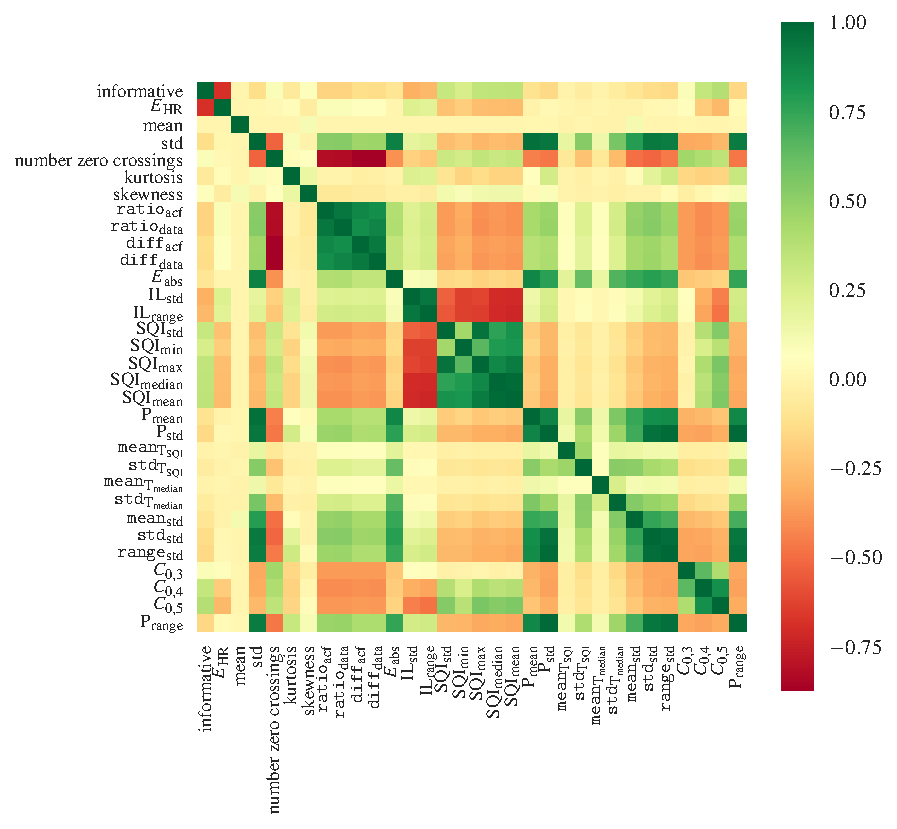
\includegraphics{pic/corr-heatmap-own.pdf}
	\caption{Korrelationsdiagramm aller entwickelten Merkmale, $E\textsubscript{HR}$ und der binären Annotation}
	\label{fig:corr-heatmap-own}
\end{figure}
 
Auch bei diesen Merkmalen wir mit dem Python-Paket \texttt{rfimp} ermittelt, welche Merkmale durch andere vorhergesagt werden können. Es zeigt sich, dass $\texttt{P}\textsubscript{min}$ und $\texttt{P}\textsubscript{max}$ sehr stark

\section{Auswahl der Modelle und Aufbau eines Basisklassifikators}

Nachdem die Merkmale entwickelt sind, werden nun Modelle ausgewählt, mit denen die Untersuchung durchgeführt wird.

Die Auswahl der Modelle beschränkt sich auf zwei Modelle, den \acl{RF} und den Gradient Boosting Tree. Beide sind ein Ensemble aus schwächeren \ac{CART}s und ermöglichen schnell trainierende, robuste Modelle, deren Entscheidung sich leicht nachvollziehen lässt und erzielen meist gute Ergebnisse. Dadurch wird eine Untersuchung der Merkmale, anhand derer die Signalqualität beurteilt werden kann, möglich.

Beide Modelle eignen sich sowohl für Regression als auch Klassifikation. Dies wird genutzt, um die Unterschiede der Ergebnisse und der Wichtigkeit der einzelnen Merkmale für beide Arten von Algorithmen zu vergleichen. Bei einer Regression kann der vorhergesagte Fehler $E\textsubscript{HR}$ mit einem Schwellwert in eine binäre Klassifikation umgewandelt werden. Dies ermöglicht einen einfachen Vergleich von Klassifikation und Regression. Damit ergeben sich insgesamt vier Lernmodelle: Jeweils Regression und Klassifikation mit einem \ac{RF} und einem Gradient Boosting Tree.

Um die Evaluation der verschiedenen Modelle zu vereinfachen, wird ein eigenständiges Basismodell entwickelt, dass das Laden der Daten, die Umwandlung der Regressionsergebnisse in eine binäre Klassifikation, das Hyperparameter-Tuning und die Evaluation der Ergebnisse bündelt.  Außerdem werden um Zuge dessen die Modelle nach dem Training serialisiert, um sie für eine  spätere Verwendung zu speichern. Dem Konstruktor dieses Basismodells werden Lernmodell, Dateiname zum Laden oder Speichern des Modells und die Hyperaramater, von denen die optimale Auswahl getroffen wird, übergeben. Wenn kein Lernmodell übergeben wird, wird automatisch versucht, die Datei mit dem übergebenen Namen zu laden. Optional kann eine Featureauswahl angegeben werden, die für das Modell verwendet werden soll. Des Weiteren werden die Eigenschaften des Datensets übergeben, das bedeutet die verwendete Segmentlänge, der Abstand in dem die Segmente erzeugt werden und der verwendete Threshold. Wurde das Datenset noch nicht erzeugt, wird dies nachgeholt. 

Sind Hyperparameter angegeben, wird das Hyperparameter-Tuning mit einer Kreuzvalidierung auf dem Trainingsset durchgeführt, wobei jeweils ein*e Patient*in zum Testen ausgelassen wird. Bei dem Hyperparameter-Tuning für die statistischen Merkmale wurde die Accuracy optimiert. Da diese bei nicht balancierten Datensets an Aussagekraft verliert und nicht zwischen Falsch-Positiven und Falsch-Negativen unterscheidet, wird hier der F1-Score optimiert.

Da bei der Erzeugung der Merkmale Lücken entstehen können, wenn für das Segment keine Intervallschätzungen existieren, werden diese Segmente unabhängig von dem verwendeten Lernmodell als nicht informativ klassifiziert. Auch beim Training werden Datenpunkte, deren Merkmale lückenhaft sind, ausgeschlossen.

Das entwickelte Basismodell ermöglicht also Hyperparameter-Tuning, Training, Vorhersage und Evaluation. Damit können auch andere Modelle und andere Daten einfach untersucht werden.






\chapter{Evaluierung der Ergebnisse}
\chapter{Zusammenfassung und Ausblick}\label{zusammenfassung}

\section{Zusammenfassung}

Ziel dieser Arbeit war die Untersuchung von Möglichkeiten, die Signalqualität von ballistokardiographischen Signalen mittels Methoden maschinellen Lernens zu beurteilen. Besonderer Fokus lag dabei bei Messdaten von bettlägerigen Patient*innen. Hierzu wurden zunächst die Grundprinzipien des maschinellen Lernens vorgestellt und die Eigenschaften von ballistokardiographischen Signalen untersucht. Auf dieser Basis wurden Besonderheiten der Signalverarbeitungen von \ac{BKG}-Signalen herausgestellt und existierende Verfahren zur Beurteilung der Signalqualität vorgestellt.

Die vorliegenden Messdaten wurden vorbereitet und ein geeignetes Verfahren zur Annotation entwickelt. Diese vorbereiteten Daten wurden anschließend genutzt, um die nachimplementierten, existierenden Verfahren zur Beurteilung der Signalqualität zu testen und zu evaluieren. Es zeigte sich, dass diese sich nur bedingt eignen, wenn die ein großer Teil des Signals von schlechter Qualität ist, wie es bei den untersuchten Daten der Fall ist. Also wurden Merkmale entwickelt, anhand derer die Signalqualität beurteilt werden kann.

Zur Untersuchung dieser Merkmale wurden insgesamt vier Modelle maschinellen Lernens ausgewählt: Regression und Klassifikation jeweils mit \acl{RF}s und Gradient Boosted Trees. Diese Modelle sind robust und schnell lernend und eignen sich somit für eine Evaluation verschiedener Einflüsse wie beispielsweise die Merkmalsauswahl, die Länge der Segmente, die beurteilt werden sollen und der Schwellwert, der für die Klassifikation verwendet wird. Um die Modelle an Besonderheiten wie Lücken in den Daten anzupassen, wurden ein eigenes Modell entwickelt, das ein Modell maschinellen Lernens erweitert. Um Regressionsverfahren für eine Klassifikation nutzen zu können, wurde auch hierfür ein Modell entwickelt, dass die Vorhersagen des Regressionsmodell in eine binäre Klassifikation umwandelt und zusätzlich Wahrscheinlichkeiten zu den Klassifikationen liefern kann.

Die Evaluierung der Modelle zeigte eine deutliche Verbesserung zu den existierenden Methoden zur Beurteilung der Signalqualität. Der Einfluss von Segmentlänge und Schwellwert der binären Annotation wurden gezeigt. Abschließend wurden die Modelle erfolgreich auf Daten einer anderen Aufnahmesituation, von schlafenden und gesunden Proband*innen, getestet.

\section{Ausblick}

Im Rahmen dieser Arbeit war es nicht Möglich, die Daten von Expert*innen annotieren zu lassen. Eine solche Annotation führt zu weniger Fehlern im zum Training verwendeten Datenset und kann so womöglich zu besseren Ergebnissen führen. Auch kann das entwickelte Merkmalsset noch um weitere Merkmale erweitert werden und unwichtigere Merkmale beispielsweise mit rekursiver Merkmalselimination verworfen werden.

Aufgrund von begrenzter Zeit und Rechenleistung wurden die Hyperparameter für diese Arbeit nur eingeschränkt optimiert. Weiteres Hyperparameter-Tuning bietet Potenzial, die Ergebnisse weiter zu verbessern. Idealerweise wird hierfür ein eigene Metrik entwickelt, die erreichte Coverage und \ac{MAE} kombiniert bewertet, da diese beiden Werte die entscheidenden für die Bewertung der Ergebnisse sind.

Auch könnte untersucht werden, ob eine Kombination von Modellen, Segmentlängen und Schwellwerten genutzt werden kann um zunächst eine gröbere Klassifikation vorzunehmen und diese anschließend zu verfeinern.






%***********************************************************
%* Anhänge			 									   *
%***********************************************************
%\addcontentsline{toc}{chapter}{Anhang}
%\appendix
%\input{./app/Dateiname}
%\chapter{Datenblätter}
%\begin{enumerate}
%      \item Datenblatt 1
%      \item Datenblatt 2
%\end{enumerate}


%***********************************************************
%* Quellenverzeichnis 									   *
%***********************************************************
\clearpage
\printbibliography[heading=bibintoc]
%\bibliographystyle{plainnat}
%\bibliography{./bib/quellen}

\end{sloppypar}
\end{document}
